% -*-mode: Latex-*-
% !TEX root = kampf.tex
% authors: simon maurer
%
% file: kampf.tex
% contents: root file with packages and includes
% Sccs-Id: %W% %G%


\documentclass[10pt, a4paper]{report}

\usepackage[utf8]{inputenc}
\usepackage[margin=1.5in]{geometry}
\usepackage{graphicx}
\usepackage{hyperref} % For hyperlinks in the PDF

%% --------------------------------------------------------------------------
%% --------------------------------------------------------------------------
%% --------------------------------------------------------------------------
\pagestyle{empty}

% add hyphen for specific words
\hyphenation{time-stamped}

% Text styles
\newcommand\textStyleSF[1]{\textit{#1}} % style used for SFs
\newcommand\textStyleM[1]{\textit{#1}}  % style used for Manöver
\newcommand\textStyleVT[1]{\textit{#1}} % style used for Vorteile
%\newcommand\textStyleAT[1]{\raisebox{10pt}{\textit{#1}}} % style used for Autotreffer/Aktionnen
\newcommand\textStyleAT[1]{\textit{#1}} % style used for Autotreffer/Aktionnen
\newcommand\textStyleTa[1]{\textit{#1}} % style used for Talente
\newcommand\textStyleStrongEmphasis[1]{\textbf{#1}}

% reanme constants
\renewcommand{\contentsname}{Inhaltsverzeichnis}
\renewcommand{\figurename}{Abbildung}

%% --------------------------------------------------------------------------
%% --------------------------------------------------------------------------
%% --------------------------------------------------------------------------

\begin{document}

% title, authors, and abstract
% -*-mode: Latex-*-
% !TEX root = paper.tex
% paper:   ...
% authors: raimund, ...
%
% file: title.tex
% contents: title, authors, and abstract
% Sccs-Id: %W% %G%

\title{
%A Survey on (Timed) Coordination Languages
Kampfregeln - kurz skizziert
  \thanks{
    %This work has been supported by ...
    Ein Regelwerk von ALRIK
    %
    % TACLE:
    % This work was partially supported by COST Action IC1202: ``Timing Analysis On Code-Level'' (TACLe).
    % This is a joint collaboration in the framework of COST Action IC1202: ``Timing Analysis On Code-Level'' (TACLe).
    %
    % SCC-MTA:
    % the Material Transfer Agreement 2010-2013 for the Intel SCC Research Processor
    % ``Light-weight Parallel Execution Layer for Stream Processing Networks
    % on Distributed Memory Architectures''.
    %
    % CRAFTERS:
    %the FP7 ARTEMIS-JU research project ``ConstRaint and Application
    %driven Framework for Tailoring Embedded Real-time Systems'' (CRAFTERS).
    %under contract no 295371.
    %
    % ADVANCE:
    %the IST FP7 research project ``Asynchronous and Dynamic
    %Virtualization through performance ANalysis to support Concurrency
    %Engineering'' (ADVANCE). %under contract no IST-2010-248828. 
    %
    % AETHER:
    %the IST FP6 research project ``Self-Adaptive, Embedded Technologies for Pervasive
    %Computer Architectures'' (AETHER). %under contract no IST-2006-027611.
    %
    % ArtistDesign: (use hyperref package for \href)
    %the European Community's Seventh Framework Programme [FP7,2008-2011] 
    %under grant agreement no 214373 (ArtistDesign, 
    %\href{http://www.artist-embedded.org/}{http://www.artist-embedded.org/}).
    %
    % SECCO:
    %the Austrian Science Fund (Fonds zur F{\"o}rderung der 
    %wissenschaftlichen Forschung) within the research project
    %``Sustaining Entire Code-Coverage on Code Optimization'' 
    %(SECCO) under contract P20944-N13.
    %
    % FORTAS:
    %the Austrian Science Fund (Fonds zur F{\"o}rderung der 
    %wissenschaftlichen Forschung) within the research project
    %``Formal Timing Analysis Suite of Real-Time Systems'' 
    %(FORTAS-RT) under contract P19230-N13.
    %
    % COSTA:
    %by the Austrian Science Fund (Fonds zur F{\"o}rderung der 
    %wissenschaftlichen Forschung) within the research project
    %``Compiler-Support for Timing Analysis'' (COSTA) under
    %contract P18925-N13.
    %
    % TEDES:
    %the FIT-IT research project ``Systematic test case generation for 
    %safety-critical distributed embedded real time systems with 
    %different SIL levels (TeDES)'';   %%under contract 809446/2297.
    %the project is carried out in cooperation with TU-Graz, 
    %Magna Steyr, and TTTech.
    %
    % ARTIST2: (use hyperref package for \href)
    %the European Community's Sixth Framework Programme [FP6/2002-2006] 
    %under grant agreement no 004527 (ARTIST2, 
    %\href{http://www.artist-embedded.org/}{http://www.artist-embedded.org/}).
    %
    % MoDECS:
    %the FIT-IT research project ``Model-Based Development of distributed 
    %Embedded Control Systems (MoDECS)'' %%under contract IST-2001-32111.
    %
    % SETTA:
    %the IST FP5 research project ``Systems Engineering for Time-Triggered 
    %Architectures (SETTA)'' under contract IST-10043.
    %
    }%\thanks
%\\\[Technical\ Report\ XX/20YY\]
%\\(Extended Abstract)
}

\author
  {
        Simon Maurer
  }

\maketitle
\thispagestyle{empty}

\begin{abstract}
Here comes the abstract...

\end{abstract}


% add page numbers in draft document
\pagestyle{headings}

% Include chapters
\tableofcontents
% -*-mode: Latex-*-
% !TEX root = paper.tex
% paper: ...
% authors: raimund, ...
%
% file: chap.intro.tex
% contents: introduction to the paper
% Sccs-Id: %W% %G%

\chapter{Einleitung}

\section{Vorwort}

\section{Wie man dieses Dokument benutzt}


% -*-mode: Latex-*-
% !TEX root = kampf.tex
% authors: simon maurer
%
% file: wunden.tex
% contents: Beschreibung der Wunden und Wundschwellen
% Sccs-Id: %W% %G%

%==============================================================================
\chapter{Wunden}
%------------------------------------------------------------------
\section{Wundschwelle}
Jeder Kämpfer hat eine Wundschwelle.
Die Wundschwelle ist KO/2, allenfalls modifiziert durch den Vorteil Eisern (+2) oder den Nachteil Glasknochen (-2).
Zu Beginn eines Kampfes würfelt jeder Kämpfer eine Selbstbeherrschungsprobe, je fünf übrigbehaltene Punkte steigt die Wundschwelle für den Kampf um 1.

Wenn die erlittenen Schadenspunkte über der Wundschwelle liegen, erleidet der Kämpfer eine Wunde.
Dadurch sinken AT, PA, FK, AW, GE um je 2 Punkte und die GS um einen Punkt.

%------------------------------------------------------------------
\section{Heilung von Wunden}
Für unbehandelte Wunden gilt: Pro Ruhephase kann ein Verwundeter eine KO-Probe ablegen, die pro Wunde um drei Punkte erschwert ist.
Gelingt diese Probe, so heilt eine Wunde.

Für behandelte Wunden (Heilkunde Wunden +3 pro Wunde) gilt: Pro Ruhephase kann ein Verwundeter eine KO-Probe ablegen, die um die Hälfte der Tap* der Heilkunde Probe erleichtert ist.
Gelingt diese Probe, so heilt eine Wunde.
Weiter gilt: Je 7 TaP* aus der Heilkunde-Probe, bei 7 eingesetzten AsP eines Balsam und für je 7 LeP, die ein magischer Heiltrank zurück gibt, heilt eine Wunde sofort.

Jede Behandlung gilt nur für die folgende Ruhephase, kann aber vor jeder Ruhephase wiederholt werden.

% -*-mode: Latex-*-
% !TEX root = kampf.tex
% authors: simon maurer
%
% file: qvat.tex
% contents: Kurze Beschreibung des QVAT Systems
% Sccs-Id: %W% %G%

%==============================================================================
\section{QVAT}
Nach QVAT gelingt jede Attacke, es sei denn man würfelt einen Patzer.
Jede Attacke hat eine Qualität.
Die Qualität berechnet sich aus der Differenz von AT-Wurf und AT-Wert geteilt durch zwei.
Liegt der AT-Wurf über dem AT-Wert, liegt eine negative Qualität vor, ansonsten eine positive.
Eine negative Qualität zählt als Parade-Erleichterung für den Verteidiger und wird vom Schaden abgezogen (Ausnahme: ein Kämpfer mit der SF Klingentänzer muss eine negative Qualität nicht vom Schaden abziehen), falls die Parade trotzdem misslingt.
Eine positive Qualität zählt als Parade-Erschwernis für den Verteidiger, modifiziert aber den Schaden nicht.

Eine Parade gelingt, wenn nicht höher als der durch die Qualität des Angreifers modifizierte PA-Wert gewürfelt wird.

% -*-mode: Latex-*-
% !TEX root = kampf.tex
% authors: simon maurer
%
% file: ini.tex
% contents: Neue Umsetzung der Initiative
% Sccs-Id: %W% %G%

%==============================================================================
\chapter{Initiative}
\label{chap.INI}
Die Initiative beeinflusst direkt die AT/PA Werte des Helden nach folgenden Regeln:
\begin{itemize}
    \item INI 0 bis 4: AT/PA -2/-2
    \item INI 5 bis 9: AT/PA -1/-1
    \item INI 10 bis 14: keine Modifikation
    \item INI 15 bis 19: AT/PA +1/+1
    \item INI 20+: AT/PA +2/+2
\end{itemize}

Der INI-Wert errechnet sich wie folgt:
\begin{itemize}
    \item INI-Basis + SF-Bonus + Waffen-Mod – BE
    \begin{itemize}
        \item INI-Basis: (MU+MU+IN+GE)/5 nach DSA4.1
        \item SF-Bonus: +4 Kampfreflexe, +2 Kampfgespür +4 Klingentänzer
        \item Waffen-Mod: INI-Modifikation der Waffe
        \item BE: effektive Behinderung (nach Verrechnung von eventuellen Rüstungsgewöhnungen)
    \end{itemize}
\end{itemize}

W6-Wurf wird also nicht dazu gezählt

% -*-mode: Latex-*-
% !TEX root = kampf.tex
% authors: simon maurer
%
% file: allgKampf.tex
% contents: Kurze Einleitung zum Kampfsystem
% Sccs-Id: %W% %G%

%==============================================================================
\chapter{Allgemeines zum Kampf}
Es gelten grundsätzlich die Regeln nach DSA4.1.
Ansagen und Erschwernisse aus Manövern senken den AT- bzw. PA-Wert, was bei der Ermittlung der Qualität relevant ist.
Manöver gelten bei negativer Qualität als misslungen und gelten als normale Attacke mit dieser negativen Qualität.
Im Gegensatz zu DSA4.1 haben misslungene Manöver keine negativen Folgewirkungen.

Es wird der Grundsatz verfolgt, nur positive Effekte in die nächste Runde mit zu nehmen (so kann niemandem vorgeworfen werden er vergesse absichtlich Modifikationen der vorherigen Runde).

% -*-mode: Latex-*-
% !TEX root = kampf.tex
% authors: simon maurer
%
% file: bAT.tex
% contents: Attacken-Manöver des bewaffneten Kampfes
% Sccs-Id: %W% %G%

%==============================================================================
\section{Bewaffnete AT-Manöver}
\label{chap.bAT}


\section{Angriff mit dem Schild}
\label{aktion.angriff_mit_dem_schild}
\textStyleAT{(Autotreffer / Aktion)}
\begin{description}
    \item[Voraussetzung:]
        SF \textStyleSF{\nameref{sf.schildkampf} I}
    \item[Probe:]
        Raufen-AT, erschwert um 3 Punkte (nicht erschwert bei Kenntnis von \textStyleSF{\nameref{sf.schildkampf} II}) und den AT-WM des Schildes (+WS)
    \item[Wirkung:]
        Wenn nichts anderes Angegeben ist, verursacht ein Schild 1W+1 TP(A) mit TP/KK 13/3.
        Ein mit Dornen ausgerüsteter Schild verursacht echte TP.
    \item[PA für den Gegner:]
        Ein Angriff mit Schild (Ausnahmen: Buckler und Bock) kann mit Dolchen, Fechtwaffen und Kettenwaffen nicht pariert werden.
        Wird der Angriff pariert entsteht auf keiner Seite Schaden.
    \item[Besonderes:]
        Kann mit einem \textStyleM{\nameref{aktion.wuchtschlag}}, einem \textStyleM{\nameref{aktion.sturmangriff}} und einem \textStyleM{\nameref{aktion.niederwerfen}} kombiniert werden.
\end{description}

\section{Auf Distanz halten}
\label{aktion.auf_distanz_halten}
\textStyleAT{(kein Autotreffer / Aktion)}
\begin{description}
    \item[Voraussetzung:]
        Distanzklasse der Waffe des Angreifers ist länger als jene des Verteidigers
    \item[Probe:]
        AT (+F)
    \item[Wirkung:]
        Der Angreifer nützt die Länge seiner Waffe aus und bringt sich so in Position, dass die die nächste Aktion des Gegners entfällt.
        Dieser Angriff verursacht kein Schaden.
    \item[Besonderes:]
        Kann mit einer \textStyleM{\nameref{aktion.finte}} kombiniert werden.
\end{description}

\subsection{Ausfall}
\label{aktion.ausfall}
\textStyleAT{(Autotreffer / Aktion)}
\begin{description}
    \item[Voraussetzung]:
        SF \textStyleSF{\nameref{sf.ausfall}}, BE \textrm{${\leq}$} 4, ausreichende Bewegungsfreiheit
    \item[Probe]:
        Einleitende AT+4, jede weitere AT normal.
        Trägt der Ausfallende ein Schild ist jede AT um (weitere) 2 Punkte erschwert (+F) (+WS)
    \item[Wirkung]:
        Der Angreifer greift mit einer Folge von Attacken an und lässt seinem Gegner keine Zeit für einen Gegenangriff, sondern drängt ihn mit jedem Schlag zurück.
        Der Ausfall endet, wenn \textStyleStrongEmphasis{eine AT eine negative Qualität} aufweist, wenn dem Gegner \textStyleStrongEmphasis{eine glückliche PA} gelingt, \textStyleStrongEmphasis{KO*AT geschlagen} wurden, der Gegner \textStyleStrongEmphasis{stehen bleibt} (MU+Qualität, bei misslingen geht Ausfall weiter, in jedem Fall PA+4), \textStyleStrongEmphasis{meisterlich pariert} (mit einer minimalen Ansage von 4) oder nicht mehr weiter zurückweichen kann (in diesem Fall PA+4 für den Verteidiger).
    \item[Besonderes]:
        Während des Ausfalls können der \textStyleM{\nameref{aktion.wuchtschlag}} und die \textStyleM{\nameref{sf.finte}} eingesetzt werden (maximale Ansage: +4).
        Als abschliessende AT ist auch ein \textStyleM{\nameref{aktion.angriff_zum_niederwerfen}}, ein \textStyleM{\nameref{aktion.hammerschlag}}, ein \textStyleM{\nameref{aktion.gezielter_stich}} oder ein \textStyleM{\nameref{aktion.todesstoss}} möglich.
\end{description}

\subsection{Befreiungsschlag}
\label{aktion.befreiungsschlag}
\textStyleAT{(Autotreffer / Aktion+Reaktion)}
\begin{description}
    \item[Voraussetzung]:
        SF \textStyleSF{\nameref{sf.befreiungsschlag}}
    \item[Probe]:
        AT+(4 pro Gegner) (+F) (+WS)
    \item[Wirkung]:
        Ein Rundumschlag, mit dem mehrere Gegner gleichzeitig angegriffen werden.
        Jeder Gegner dem die PA misslingt erleidet einen Treffer, und verliert die folgende AT.
        Können die Gegner aus irgendwelchen Gründen nicht zurückweichen, erleiden sie 1W6 Punkte zusätzlichen Schaden.
    \item[Besonderes]:
        Kann mit einem \textStyleM{\nameref{aktion.wuchtschlag}} und einer \textStyleM{\nameref{aktion.finte}} kombiniert werden.
\end{description}

\subsection{Betäubungsschlag}
\label{aktion.betaeubungsschlag}
\textStyleAT{(Autotreffer / Aktion)}
\begin{description}
    \item[Voraussetzung]:
        SF \textStyleSF{\nameref{sf.betaeubungsschlag}}, Waffe mit stumpfer Seite
    \item[Probe]:
        Kampfstäbe, stumpfe Hiebwaffen AT+2, stumpfe Seiten anderer Hiebwaffen AT+4, andere mögliche Waffen AT+8, mit Knauf Raufen-AT+4 (+WS)
    \item[Wirkung]:
        Ein starker Schlag, der den Gegner bewusstlos schlagen soll, ohne diesen schwer zu verletzen.
        Der Schlag richtet keine richtigen TP sondern nur TP(A) an.
        Übersteigen die TP(A) die Wundschwelle des Gegners, muss dieser eine KO-Probe ablegen.
        Bei Misslingen, fällt das Opfer für 1W6 SR in Ohnmacht.
        Übersteigen die TP(A) gar die KO, so steht dem Gegner keine KO-Probe zu.
    \item[Besonderes]:
        Kann mit einem \textStyleM{\nameref{aktion.wuchtschlag}} kombiniert werden, die Ansage kann zur TP-Steigerung oder als KO-Erschwernis eingesetzt werden.
\end{description}

\subsection{Doppelangriff}
\label{aktion.doppelangriff}
\textStyleAT{(Autotreffer / Aktion)}
\begin{description}
    \item[Voraussetzung]:
        SF \textStyleSF{\nameref{sf.doppelangriff}}, zwei Einhand-Waffen die in der gleichen DK verwendbar sind, keine Kettenwaffen und Speere
    \item[Probe]:
        AT+2 pro Hand, bei nicht identischen Waffen Zweithand zusätzlich +4, Zweithand zusätzlich +3 ohne die SF \textStyleSF{\nameref{sf.beidhaendiger_kampf} II}
    \item[Wirkung]:
        Mit beiden Waffen wird gleichzeitig zugeschlagen.
        Es werden zwei Paraden benötigt (\textStyleM{\nameref{reaktion.defensiver_kampfstil}}, \textStyleM{\nameref{reaktion.klingenwand}}, PA und Gezieltes Ausweichen, PA und zusätzliche PA von Zweitwaffe).
\end{description}

\subsection{Entwaffnen}
\label{aktion.entwaffnen}
\textStyleAT{(kein Autotreffer / Aktion)}
\begin{description}
    \item[Voraussetzung]:
        SF \textStyleSF{\nameref{sf.entwaffnen}}
    \item[Probe]:
        AT+8 (+F)
    \item[Wirkung]:
        Dieser schnelle Angriff zielt nicht auf eine Verletzung ab, sondern soll den Gegner entwaffnen.
        Misslingt die PA des Verteidigers, muss er eine KK-Probe erschwert um 8 (um 10 bei Kenntnis der SF \textStyleSF{\nameref{sf.meisterliches_entwaffnen}}) bestehen, sonst verliert er die Waffe.
        Bei diesem Angriff entsteht beim Getroffenen kein Schaden.
    \item[Besonderes]:
        Mit Kampfstäben ist dieses Manöver um 2 Punkte, mit Kettenstäben und Zweililien um 4 Punkte erleichtert.
        Entwaffnen ist üblicherweise nur gegen einhändig geführte Waffen möglich.
        Wer allerdings die SF \textStyleSF{\nameref{sf.meisterliches_entwaffnen}} beherrscht, kann auch Gegner mit Zweihandwaffen entwaffnen.
        Das Vorgehen entspricht dem, was auch bei Einhandwaffen gilt.
    \item[Besonderes]:
        Kann mit einer \textStyleM{\nameref{aktion.finte}} kombiniert werden, die Ansage kann als PA-Erschwernis oder KK-Erschwernis eingesetzt werden.
\end{description}

\section{Festnageln}
\label{aktion.festnageln}
\textStyleAT{(Autotreffer / Aktion+Reaktion)}
\begin{description}
    \item[Voraussetzung:]
        SF \textStyleSF{\nameref{sf.festnageln}}, Stangenwaffe oder Speer mit gerader Klinge und einem Knebel, der ein zu tiefes eindringen der Klinge verhindert.
    \item[Probe, Wirkung:]
        Siehe S. 62 WdS.
\end{description}

\subsection{Finte}
\label{aktion.finte}
\textStyleAT{(Autotreffer / Aktion)}
\begin{description}
    \item[Voraussetzung]:
        BE\textrm{ ${\leq}$ }4
    \item[Probe]:
        AT+Ansage (+WS)
    \item[Wirkung]:
        Der Angreifer täuscht einen Schlag auf eine bestimmte Körperzone an, um dann die Waffe umzulenken und an einer anderen Stelle zu treffen.
        Die Attacke erschwert um eine Ansage ergibt einen Qualitätsbonus in Höhe der Ansage, bei Kenntnis der SF \textStyleSF{\nameref{sf.finte}} sogar einen Qualitätsbonus in Höhe der doppelten Ansage.
    \item[Besonderes]:
        Kann mit einem \textStyleM{\nameref{aktion.wuchtschlag}} kombiniert werden.
\end{description}

\section{Gezielter Stich}
\label{aktion.gezielter_stich}
\textStyleAT{(Autotreffer / Aktion)}
\begin{description}
    \item[Voraussetzung:]
        SF \textStyleSF{\nameref{sf.gezielter_stich}}
    \item[Probe:]
        AT+4 + halber gegnerischer RS (+F)
    \item[Wirkung:]
        Diese Attacke richtet sich gezielt gegen eine verwundbare, ungerüstete Stelle des Gegners.
        Erstens wird die Rüstung des Gegners ignoriert (auch natürlicher RS), zweitens ist seine Wundschwelle bei dieser Art von Angriff um 2 Punkte gesenkt und drittens erleidet er automatisch eine Wunde.
    \item[Besonderes:]
        Kann mit einer \textStyleM{\nameref{aktion.finte}} kombiniert werden.
\end{description}

\subsection{Hammerschlag}
\label{aktion.hammerschlag}
\textStyleAT{(Autotreffer / Aktion+alle Reaktionen)}
\begin{description}
    \item[Voraussetzung]:
        SF \textStyleSF{\nameref{sf.hammerschlag}}
    \item[Probe]:
        AT+8 (+WS) (+F)
    \item[Wirkung]:
        Mit diesem riskanten und mit aller Kraft geführten Schlag versucht der Kämpfer, den Kampf möglichst mit einem einzelnen Schlag zu beenden.
        Die TP werden verdreifacht (das beinhaltet auch TP/KK und allfällige Ansage aus \textStyleM{\nameref{aktion.wuchtschlag}}).
    \item[Besonderes]:
        Kann mit einem \textStyleM{\nameref{aktion.wuchtschlag}} und einer \textStyleM{\nameref{aktion.finte}} (wenn die Waffe eine Finte erlaubt) kombiniert werden.
\end{description}

\subsection{Klingensturm}
\label{aktion.klingensturm}
\textStyleAT{(Autotreffer / Aktion)}
\begin{description}
    \item[Voraussetzung]:
        SF \textStyleSF{\nameref{sf.klingensturm}}, Kämpfer führt keinen Schild, BE\textrm{ ${\leq}$ }4
    \item[Probe]:
        Zwei AT gegen zwei unterschiedliche Gegner, jeweils auf (AT/2)+2.\newline
        Bei Kenntnis der SF \textStyleSF{\nameref{sf.kampfgespuer}} können AT+4 Punkte frei auf zwei AT gegen zwei Gegner verteilt werden, wobei der Mindestwert einer AT 6 beträgt.\newline
        Bei Kenntnis der SF \textStyleSF{\nameref{sf.klingentaenzer}} können AT+6 Punkte frei auf drei AT gegen drei Gegner verteilt werden, wobei der Mindestwert einer AT 6 beträgt.
    \item[Wirkung]:
        Mit dieser Attacke kann eine Kämpferin zwei Gegner in direkter Folge angreifen, also mit einem einzigen Angriffsmanöver.
\end{description}

\subsection{Niederwerfen}
\label{aktion.niederwerfen}
\textStyleAT{(Autotreffer / Aktion)}
\begin{description}
    \item[Voraussetzung]:
        SF \textStyleSF{\nameref{sf.niederwerfen}}
    \item[Probe]:
        AT+4(+Ansage) (+WS)
    \item[Wirkung]:
        Der Schlag verursacht Schaden wie üblich.
        Zusätzlich muss der Gegner eine KK-Probe, erschwert um eine allfällige Ansage, Erleichterungen für \textStyleSF{Standfest} (-1), \textStyleVT{Balance} (-2), \textStyleVT{Herausragende Balance} (-4) bestehen um auf den Beinen zu bleiben.
    \item[Besonderes]:
        Kann mit einem \textStyleM{\nameref{aktion.sturmangriff}} und einem \textStyleM{\nameref{aktion.wuchtschlag}} kombiniert werden.
\end{description}

\subsection{Passierschlag}
\label{aktion.passierschlag}
\textStyleAT{(kein Autotreffer / Freie Raufen oder Ringen-Aktion)}
\begin{description}
    \item[Voraussetzung]:
        Ein Kämpfer durchschreitet den eigenen Kontrollbereich oder gibt sich durch eine Aktion eine Blösse
    \item[Probe]:
        AT+4
    \item[Wirkung]:
        Als Freie Aktion kann einem unvorsichtigen Kämpfer, der den eigenen Kontrollbereich durchschritten oder sich durch ein Manöver in eine unglückliche Lage begeben hat (Sturmangriff) ein ungezielter Schlag versetzt werden (keine Manöver).
        Besitzt das Opfer die SF \textStyleSF{\nameref{sf.aufmerksamkeit}} ist der Schlag um weitere 4 Punkte erschwert, bei der SF \textStyleSF{\nameref{sf.kampfgespuehr}} gar um 6 Punkte (4 aus \textStyleSF{\nameref{sf.aufmerksamkeit}} und 2 aus \textStyleSF{\nameref{sf.kampfgespuehr}}).
\end{description}

\section{Schildspalter}
\label{aktion.schildspalter}
\textStyleAT{(kein Autotreffer / Aktion)}
\begin{description}
    \item[Voraussetzung:]
        SF \textStyleSF{\nameref{sf.schildspalter}}
    \item[Probe:]
        AT+8(+Ansage), erleichtert um PA-WM des Schildes
    \item[Wirkung:]
        Mit einer geeigneten Waffe ist es möglich, den Schild einer Gegnerin zu spalten oder so zu verbeulen, dass er jeden Nutzen verliert.
        Misslingt die Parade des Verteidigers, muss er einen Bruchfaktortest erschwert um eine allfällige Ansage würfeln.
\end{description}

\subsection{Stumpfer Schlag}
\label{aktion.stumpfer_schlag}
\textStyleAT{(Autotreffer / Aktion)}
\begin{description}
    \item[Voraussetzung]:
        keine
    \item[Probe]:
        Kampfstäbe, stumpfe Hiebwaffen AT+2, stumpfe Seiten anderer Hiebwaffen AT+4, andere mögliche Waffen AT+8, mit Knauf Raufen-AT+4.
        Bei Kenntnis der SF \textStyleSF{\nameref{sf.betaeubungsschlag}}, werden die genannten AT-Zuschläge halbiert.
    \item[Wirkung]:
        Der Angreifer schlägt gebremst oder mit der flachen Seite der Waffe zu, um möglichst wenig realen Schaden, sondern nur Betäubungsschaden zu verursachen.
        Solche Schläge richten TP(A) statt TP an.
\end{description}

\section{Sturmangriff}
\label{aktion.sturmangriff}
\textStyleAT{(kein Autotreffer / speziell)}
\begin{description}
    \item[Voraussetzung:]
        SF \textStyleSF{\nameref{sf.sturmangriff}}, wenigstens 4 Schritt Anlauf, GS\textrm{ ${\geq}$ 4}
    \item[Probe:]
        AT+4 (+WS)
    \item[Wirkung:]
        Ein Angriff mit Anlauf, der durch den Schwung des Kämpfers mehr Schaden verursachen soll.
        Die halbe Geschwindigkeit wird als TP-Bonus zum Schaden addiert.
        Dazu zusätzlich 4 Punkte und eine allfällige Ansage.
        Misslingt das Manöver, so entfällt die Reaktion des Angreifers und der Verteidiger kann einen Passierschlag ausführen.
    \item[Besonderes:]
        Kann mit einem \textStyleM{\nameref{aktion.niederwerfen}} und einem \textStyleM{\nameref{aktion.wuchtschlag}} kombiniert werden.
\end{description}

\subsection{Tod von Links}
\label{aktion.tod_von_links}
\textStyleAT{(Autotreffer / Aktion)}
\begin{description}
    \item[Voraussetzung]:
        SF \textStyleSF{\nameref{sf.tod_von_links}}, BE\textrm{ ${\leq}$ }4
    \item[Probe]:
        AT mit dem AT-Wert der Parierwaffe, zusätzlich +3 ohne SF \textStyleSF{\nameref{sf.beidhaendiger_kampf} II} (+F)
    \item[Wirkung]:
        Eine zusätzliche Attacke mit der falschen Hand (nicht kumulierbar mit einer Zusatzaktion aus \textStyleSF{\nameref{sf.beidhaendiger_kampf} II}), die mit der Parierwaffe ausgeführt werden muss.
    \item[Besonderes]:
        Kann mit einer \textStyleM{\nameref{aktion.finte}} kombiniert werden.
\end{description}

\subsection{Todesstoss}
\label{aktion.todesstoss}
\textStyleAT{(Autotreffer / Aktion+alle Reaktionen)}
\begin{description}
    \item[Voraussetzung]:
        SF \textStyleSF{\nameref{sf.todesstoss}}
    \item[Probe]:
        AT+8 + halber gegnerischer RS (+F) (+WS)
    \item[Wirkung]:
        Eine riskante Version des gezielten Stichs, mit dem der Gegner mit einem einzigen Stich kampfunfähig gemacht werden soll.
        Der RS wird ignoriert (nicht aber natürlicher RS).
        Um die SP zu ermitteln wird der Schaden (Waffen-Schaden inklusive KK-Bonus) verdoppelt.
        Die Wundschwelle des Verteidigers ist um 2 reduziert und es werden automatisch zwei Wunden verursacht.
    \item[Besonderes]:
        Kann mit einer \textStyleM{\nameref{aktion.finte}} und einem \textStyleM{\nameref{aktion.wuchtschlag}} (selbst wenn die Waffe keinen \textStyleM{\nameref{aktion.wuchtschlag}} erlauben würde) kombiniert werden.
\end{description}

\subsection{Umreissen}
\label{aktion.umreissen}
\textStyleAT{(kein Autotreffer / Aktion)}
\begin{description}
    \item[Voraussetzung]:
        SF \textStyleSF{\nameref{sf.umreissen}}, Kämpfer führt weder Schild noch Parierwaffe
    \item[Probe]:
        AT+8 (+F)
    \item[Wirkung]:
        Bei dieser Variante der \textStyleM{\nameref{aktion.finte}} soll der Gegner durch geschickte Platzierung des Treffers zu Boden gezwungen werden.
        Kann nicht Pariert werden, muss das Opfer eine um die TP des Angriffs erschwerte GE Probe bestehen um auf den Beinen zu bleiben (Erleichterungen für \textStyleSF{Standfest} (-2), \textStyleVT{Balance} (-4) und \textStyleVT{Herausragende Balance} (-8)).
        Ein Treffer erzeugt keinen Schaden.
    \item[PA für den Gegner]:
        Der Angriff kann nur mit einer PA+8, einer \textStyleTa{Raufen}- oder \textStyleTa{Ringen}-PA mit \textStyleSF{\nameref{sf.beinarbeit}} oder mit einem Ausweichen pariert werden.
    \item[Besonderes]:
        Kann mit einer \textStyleM{\nameref{aktion.finte}} kombiniert werden.
\end{description}

\section{Unterlaufen}
\label{aktion.unterlaufen}
\textStyleAT{(kein Autotreffer / Aktion)}
\begin{description}
    \item[Voraussetzung:]
        Distanzklasse der Waffe des Angreifers ist kürzer als jene des Verteidigers
    \item[Probe:]
        AT+4 (+F)
    \item[Wirkung:]
        Diese Verzweiflungstat erlaubt dem Angreifer eine kurze Verschnaufpause, bis der Verteidiger ihn wieder von sich weggestossen hat.
        Der Angreifer nützt die Kürze seiner Waffe aus und unterläuft den Gegner.
        Die nächste Aktion des Gegners entfällt.
        Dieser Angriff verursacht kein Schaden.
    \item[Besonderes:]
        Kann mit einer \textStyleM{\nameref{aktion.finte}} kombiniert werden.
\end{description}

%------------------------------------------------------------------

\subsection{Wuchtschlag}
\label{aktion.wuchtschlag}
\textStyleAT{(Autotreffer / Aktion)}
\begin{description}
    \item[Voraussetzung]:
        keine
    \item[Probe]:
        AT+Ansage (+F)
    \item[Wirkung]:
        Der Kämpfer führt einen besonders kraftvollen Schlag aus.
        Die TP werden um die hälfte der Ansage erhöht.
        Bei Kenntnis der SF \textStyleSF{\nameref{sf.wuchtschlag}} werden die TP gar um die ganze Ansage erhöht.
    \item[Besonderes]:
        Kann mit einer \textStyleM{\nameref{aktion.finte}} kombiniert werden.
\end{description}


% -*-mode: Latex-*-
% !TEX root = kampf.tex
% authors: simon maurer
%
% file: bPA.tex
% contents: Paraden-Manöver des bewaffneten Kampfes
% Sccs-Id: %W% %G%

%==============================================================================
\section{Bewaffnete PA-Manöver}
\label{chap.bPA}

\subsection{Binden}
\label{reaktion.binden}
\begin{description}
    \item[Voraussetzung]:
        SF \textStyleSF{\nameref{sf.binden}}
        \begin{itemize}
            \item
                Mit Hauptwaffe + \textStyleSF{\nameref{sf.meisterparade}}:\newline
                Probe: +Ansage des Gegners, mindestens +4 + Ansage\newline
                Wirkung: erleichtert die nächste Aktion um die Ansage und erhöht die Qualität der nächsten Aktion um die Ansage.
            \item
                Mit \textStyleSF{\nameref{sf.parierwaffen}}:\newline
                Probe: +Ansage des Gegners, mindestens +4\newline
                Wirkung: erleichtert die nächste Aktion um 4 und erhöht die Qualität der nächsten Aktion um 4
            \item
                Mit Hauptwaffe + \textStyleSF{\nameref{sf.meisterparade}} und \textStyleSF{\nameref{sf.parierwaffen}}:\newline
                Probe: +Ansage des Gegners, mindestens +4 +Ansage\newline
                Wirkung: erleichtert nächste die Aktion um 4+Ansage und erhöht die Qualität der nächsten Aktion um 4+Ansage
        \end{itemize}
\end{description}

\section{Defensiver Kampfstil}
\label{reaktion.defensiver_kampfstil}
\begin{description}
    \item[Voraussetzung:]
        SF \textStyleSF{\nameref{sf.defensiver_kampfstil}}
    \item[Probe:]
        normale PA
    \item[Wirkung:]
        Zwei PA anstelle einer PA und einer AT.
\end{description}

\section{Entwaffnen}
\label{reaktion.entwaffnen}
\begin{description}
    \item[Voraussetzung:]
        SF \textStyleSF{\nameref{sf.entwaffnen}}
    \item[Probe:]
        PA+8
    \item[Wirkung:]
        Gelingt die PA des Verteidigers, muss der Angreifer eine KK-Probe erschwert um 8 (um 10 bei Kenntnis der SF \textStyleSF{\nameref{sf.meisterliches_entwaffnen}}) bestehen, sonst verliert er die Waffe.
    \item[Besonderes:]
        Mit Bock, Hakendolch, Linkhand und ev. Drachenklaue ist dieses Manöver um 2 Punkte erleichtert (benötigt Kenntnis der SF \textStyleSF{\nameref{sf.parierwaffen} I}).
        Entwaffnen ist üblicherweise nur gegen einhändig geführte Waffen möglich.
        Wer allerdings die SF \textStyleSF{\nameref{sf.meisterliches_entwaffnen}} beherrscht, kann auch Gegner mit Zweihandwaffen entwaffnen.
        Das Vorgehen entspricht dem, was auch bei Einhandwaffen gilt.
    \item[Besonderes:]
        Eine zusätzliche Ansage kann als KK-Erschwernis eingesetzt werden.
\end{description}

\section{Formation}
\label{reaktion.formation}
\begin{description}
    \item[Voraussetzung:]
        SF \textStyleSF{\nameref{sf.formation}}
    \item[Probe:]
        normale PA
    \item[Wirkung:]
        Es ist möglich ohne Probenerschwernis für einen Kameraden zu parieren, so sich dieser in unmittelbarer Nähe befindet.
\end{description}

\section{Gegenhalten}
\label{reaktion.gegenhalten}
\begin{description}
    \item[Voraussetzung:]
        SF \textStyleSF{\nameref{sf.gegenhalten}}
    \item[Probe:] AT +4
    \item[Wirkung:]
        Derjenige mit der besseren Qualität macht vollen Schaden, derjenigen mit der schlechteren nur den halben.
        Bei gleicher Güte gewinnt der ursprüngliche Angreifer.
        Eine negative Qualität wird wie üblich vom Schaden abgezogen (gegebenenfalls zuerst halbieren).
\end{description}

\section{Klingenwand}
\label{reaktion.klingenwand}
\begin{description}
    \item[Voraussetzung:] SF \textStyleSF{\nameref{sf.klingenwand}}, Kämpfer führt keinen Schild, BE\textrm{ ${\leq}$ }4
    \item[Probe:]
        Zwei PA gegen zwei unterschiedliche Gegner, jeweils auf (PA/2)+2.
        \begin{itemize}
            \item Bei Kenntnis der SF \textStyleSF{\nameref{sf.kampfgespuer}} können PA+4 Punkte frei auf zwei PA gegen zwei Gegner verteilt werden, wobei der Mindestwert einer PA 6 beträgt.
            \item Bei Kenntnis der SF \textStyleSF{\nameref{sf.klingentaenzer}} können PA+6 Punkte frei auf drei PA gegen drei Gegner verteilt werden, wobei der Mindestwert einer PA 6 beträgt.
            Ein \textStyleSF{\nameref{sf.klingentaenzer}} darf mit der PA-Aufteilung warten bis die Gegner ihre AT gwürfelt haben.
        \end{itemize}
    \item[Wirkung:]
        Mit dieser Parade kann eine Kämpferin zwei Angriffe in direkter Folge parieren, also mit einem einzigen Parademanöver.
\end{description}

\subsection{Meisterparade}
\label{reaktion.meisterparade}
\begin{description}
    \item[Voraussetzung]:
    SF \textStyleSF{\nameref{sf.meisterparade}}, BE\textrm{ ${\leq}$ }4, \textStyleSF{\nameref{sf.meisterparade}} mit Schild nur bei Kenntnis der SF \textStyleSF{\nameref{sf.schildkampf} II}
    \item[Probe]:
        PA + Ansage
    \item[Wirkung]:
        Parade erschwert um Ansage ergibt eine Erleichterung der nächsten Aktion in Höhe der Ansage.
\end{description}

\section{Unterlaufen}
\label{reaktion.unterlaufen}
\begin{description}
    \item[Voraussetzung:]
        Distanzklasse der Waffe des Verteidigers ist kürzer als jene des Angreifers
    \item[Probe:]
        PA+8
    \item[Wirkung:]
        Bei dieser waghalsigen Aktion nützt der Verteidiger die Kürze seiner Waffe aus und unterläuft den Gegner.
        Die nächste Reaktion des Gegners entfällt.
        Kennt der Gegner die SF \textStyleSF{\nameref{sf.halbschwert}}, kann er trotz dem Unterlaufen dennoch parieren (ohne Einsatz eines anderen Manövers).
\end{description}

\section{Waffe Zerbrechen}
\label{reaktion.waffe_zerbrechen}
\begin{description}
    \item[Voraussetzung:]
        SF \textStyleSF{\nameref{sf.waffe_zerbrechen}}, nur gegen Klingenwaffen
    \item[Probe:]
        PA +8
    \item[Wirkung:]
        Wenn dem Verteidiger die PA gelingt, dann muss er eine KK-Probe ablegen (Erschwernisse je nach Waffe, erleichter um BF der gegnerischen Waffe).
        Bei Gelingen zerbricht die Waffe des Gegners.
        Dieser hat die Möglichkeit seine Waffe fallen zu lassen um zu verhindern, dass sie zerbricht.
\end{description}

\section{Windmühle}
\label{reaktion.windmuehle}
\begin{description}
    \item[Voraussetzung:]
        SF \textStyleSF{\nameref{sf.windmuehle}}, Kämpfer trägt kein grosser oder sehr grosser Schild, der zu konternde Angriff ist ein \textStyleM{\nameref{aktion.wuchtschlag}}, \textStyleM{\nameref{aktion.hammerschlag}}, \textStyleM{\nameref{aktion.sturmangriff}} oder \textStyleM{\nameref{aktion.befreiungsschlag}}
    \item[Probe:]
        PA +8
    \item[Wirkung:]
        Dieses gewagte Manöver setzt die Wucht des gegnerischen Hiebes in eine eigene Angriffs-Aktion um.
        Gelingt die Windmühle, so gilt sie gleichzeitig als gelungener Wuchtschlag +8.
        Dieser kann mit einer Parade (keine Manöver möglich, verbraucht keine Aktion), erschwert um die Erschwernis des ursprünglichen Angriffmanövers (plus zusätzlich die Qualität der Windmühle) abgewehrt werden.
\end{description}


% -*-mode: Latex-*-
% !TEX root = kampf.tex
% authors: simon maurer
%
% file: fkM.tex
% contents: Manöver für den Fernkampf
% Sccs-Id: %W% %G%

%==============================================================================

\chapter{Fernkampf Manöver}
\label{chap.fkM}

\section{Ansage}
\label{fkM.ansage}
\textStyleAT{(kein Autotreffer / mehrere Aktionen)}
\begin{description}
    \item[Voraussetzung:]
        keine
    \item[Probe:]
        FK+Ansage
    \item[Wirkung:]
        Der Kämpfer führt einen besonders gut gezielten Wurf / Schuss aus.
        Die TP werden um die Hälfte der Ansage erhöht.
        Dabei müssend halb so viele zusätzliche Aktionen aufgewendet werden wie der gewünschte Zuschlag beträgt.

        Bei Kenntnis der SF \textStyleSF{\nameref{sf.scharfschuetze}} werden die TP um die ganze Ansage erhöht und es müssen zwei Aktionen weniger zum Zielen aufgewendet werden (mindestens jedoch eine zusätzliche Aktion).

        Bei Kenntnis der SF \textStyleSF{\nameref{sf.meisterschuetze}} werden die TP um die ganze Ansage erhöht und es muss nur eine Aktion zum Zielen aufgewendet werden.
\end{description}

\section{Eisenhagel}
\label{fkM.eisenhagel}
\textStyleAT{(kein Autotreffer / Aktion)}
\begin{description}
    \item[Voraussetzung:]
        SF \textStyleSF{\nameref{sf.eisenhagel}}, nur mit Wurfsternen, -scheiben oder -ringen
    \item[Probe:]
        FK+2*Anzahl der Geschosse (maximal 5) +5 pro zusätzlichem Ziel
    \item[Wirkung:]
        Es werden mehrere Geschosse gleichzeitig geworfen. Ihre TP werden einzeln ermittelt.
\end{description}

\section{Schnellschuss}
\label{fkM.schnellschuss}
\textStyleAT{(kein Autotreffer / freie Aktion)}
\begin{description}
    \item[Voraussetzung:]
        Wurfwaffe in der Hand, Schusswaffe gespannt, Ziel nicht weiter als 10 Schritt entfernt
    \item[Probe:]
        FK+2
    \item[Wirkung:]
        Der Schuss / Wurf wird ungezielt auf das Ziel abgegeben.
        Dadurch benötigt der Schütze / Werfer auch keine Aktion zum Zielen.
        Bei Kenntnis der SF \textStyleSF{\nameref{sf.scharfschuetze}} ist die Probe nur um einen Punkt erschwert und bei Kenntnis der SF \textStyleSF{\nameref{sf.meisterschuetze}} entfällt der Aufschlag ganz.
\end{description}

\section{Zielen}
\label{fkM.zielen}
\textStyleAT{(kein Autotreffer / mehrere Aktionen)}
\begin{description}
    \item[Voraussetzung:]
        keine
    \item[Probe:]
        FK - Erleichterung
    \item[Wirkung:]
        Durch langes Zielen kann für zwei zusätzlich aufgewendete Aktionen der Zuschlag auf die Fernkampf-Probe um einen Punkt reduziert werden.
        Es können auf diese Art maximal 4 Punkte Erschwernis abgebaut werden.
        Bei Kenntnis der SF \textStyleSF{\nameref{sf.scharfschuetze}} oder \textStyleSF{\nameref{sf.meisterschuetze}} muss nur eine Aktion aufgewendet werden um die Erschwernis um einen Punkt zu reduzieren.
\end{description}


% -*-mode: Latex-*-
% !TEX root = kampf.tex
% authors: simon maurer
%
% file: uAT.tex
% contents: Unbewaffnete Attacke Manöver
% Sccs-Id: %W% %G%

%==============================================================================

\chapter{Unbewaffnete AT-Manöver}
\label{chap.uAT}

\section{Doppelschlag}
\label{uAT.doppelschlag}
\textStyleAT{(Autotreffer / Raufen-Aktion)}
\begin{description}
    \item[Voraussetzung:]
        SF \textStyleSF{\nameref{sf.doppelschlag}}
    \item[Probe:]
        AT+2 pro Hand, Zweithand zusätzlich +3 ohne \textStyleSF{\nameref{sf.beidhaendiger_kampf} II}
    \item[Wirkung:]
        Dies ist das waffenlose Manöver des \textStyleM{\nameref{bAT.doppelangriff}s}:
        Mit beiden Händen wird gleichzeitig zugeschlagen.
        Es werden zwei Paraden benötigt (PA und Gezieltes Ausweichen, PA und zusätzliche PA von Zweithand).
\end{description}

\section{Fussfeger}
\label{uAT.fussfeger}
\textStyleAT{(kein Autotreffer / Raufen-Aktion)}
\begin{description}
    \item[Voraussetzung:]
        SF \textStyleSF{\nameref{sf.fussfeger}}
    \item[Probe:]
        AT+8 (+F)
    \item[Wirkung:]
        Dies ist das waffenlose Manöver des \textStyleM{\nameref{bAT.umreissen}s}:
        Kann nicht Pariert werden, muss das Opfer eine um die TP(A) des Angriffs erschwerte GE Probe bestehen um auf den Beinen zu bleiben (Erleichterungen für \textStyleSF{Standfest} (-2), \textStyleSF{Balance} (-4) und \textStyleSF{Herausragende Balance} (-8)).
        Ein Treffer erzeugt keinen Schaden. 
    \item[PA für den Gegner:]
        Der Angriff kann nur mit einer Waffen-PA+8, einer Raufen- oder Ringen-PA mit \textStyleSF{\nameref{sf.beinarbeit}} oder mit einem \textStyleSF{\nameref{sf.ausweichen}} pariert werden.
    \item[Besonderes:]
        Kann mit einem \textStyleM{\nameref{uAT.schwinger}} kombiniert werden.
\end{description}


\section{Griff}
\label{uAT.griff}
\textStyleAT{(kein Autotreffer / Ringen-Aktion)}
\begin{description}
    \item[Voraussetzung:]
        SF \textStyleSF{\nameref{sf.griff}}
    \item[Probe:]
        AT +Ansage (+F)
    \item[Wirkung:]
        Ein Griff soll den Gegner kampfunfähig machen und zielt nicht darauf ab, Schaden zu verursachen.
        Kann der Angriff nicht Pariert werden, ist jede folgende Aktion des Gegriffenen um die doppelte Ansage erschwert.
        Der Griff hält an, bis der Greifende freiwillig loslässt oder der Gegriffene sich befreien kann:
        Der Gegriffene kann versuchen, den Griff mit einer (nicht erschwerten) Raufen oder Ringen-AT abzuschütteln, die wiederum vom Greifenden mit einer normalen Ringen-PA pariert werden kann.
    \item[Besonderes:]
        Kann mit einem \textStyleSF{\nameref{sf.schwinger}} kombiniert werden.
\end{description}

\section{Knochenbrecher}
\label{uAT.knochenbrecher}
\textStyleAT{(Autotreffer / Raufen- oder Ringen-Aktion)}
\begin{description}
    \item[Voraussetzung:]
        keine
    \item[Probe:]
        AT+Ansage (+F)
    \item[Wirkung:]
        Dies ist das waffenlose Manöver des \textStyleM{\nameref{bAT.wuchtschlag}s}:
        Der Kämpfer führt einen besonders kraftvollen Schlag aus.
        Die TP(A) werden um die Hälfte der Ansage erhöht.
        Bei Kenntnis der SF \textStyleSF{\nameref{sf.knochenbrecher}} werden die TP gar um die ganze Ansage erhöht.
    \item[Besonderes:]
        Kann mit einem \textStyleM{\nameref{uAT.schwinger}} kombiniert werden.
\end{description}

\section{Niederschlagen/-werfen}
\label{uAT.niederschlagen}
\textStyleAT{(Autotreffer / Raufen- oder Ringen-Aktion)}
\begin{description}
    \item[Voraussetzung:]
        SF \textStyleSF{\nameref{sf.knochenbrecher}}
    \item[Probe:]
        AT+4(+Ansage) (+WS)
    \item[Wirkung:]
        Dies ist das waffenlose Manöver des \textStyleM{\nameref{bAT.niederwerfen}s}.
        Das Manöver verursacht Schaden wie üblich. Zusätzlich muss der Gegner eine KK-Probe, erschwert um eine allfällige Ansage, Erleichterungen für \textStyleSF{Standfest} (-1), \textStyleSF{Balance} (-2), \textStyleSF{Herausragende Balance} (-4) bestehen um auf den Beinen zu bleiben.
        Beherrscht der Angreifer die SF \textStyleSF{\nameref{sf.wurf} (nur Ringen)} und wurde der Verteidiger zuvor mit dem Manöver \textStyleM{\nameref{uAT.griff}} gegriffen, so steht dem Verteidiger keine Probe zum Stehenbleiben zu.
    \item[Besonderes:]
        Kann mit einem \textStyleSF{\nameref{uAT.sprungtritt}} und einem \textStyleSF{\nameref{uAT.knochenbrecher}} kombiniert werden.
\end{description}


\section{Passierschlag}
\label{uAT.passierschlag}
\textStyleAT{(kein Autotreffer / Freie Raufen oder Ringen-Aktion)}
\begin{description}
    \item[Voraussetzung:]
        Ein Kämpfer durchschreitet den eigenen Kontrollbereich oder gibt sich durch eine Aktion eine Blösse
    \item[Probe:]
        AT+4
    \item[Wirkung:]
        Als Freie Aktion kann einem unvorsichtigen Kämpfer, der den eigenen Kontrollbereich durchschritten oder sich durch ein Manöver in eine unglückliche Lage begeben hat (Sturmangriff) ein ungezielter Schlag versetzt werden (keine Manöver).
        Besitzt das Opfer die SF \textStyleSF{\nameref{sf.aufmerksamkeit}} ist der Schlag um weitere 4 Punkte erschwert, bei der SF \textStyleSF{\nameref{sf.kampfgespuer}} gar um 6 Punkte (4 aus \textStyleSF{\nameref{sf.aufmerksamkeit}} und 2 aus \textStyleSF{\nameref{sf.kampfgespuer}}).
\end{description}

\section{Schmetterschlag}
\label{uAT.schmetterschlag}
\textStyleAT{(Autotreffer / Raufen-Aktion)}
\begin{description}
    \item[Voraussetzung:]
        SF \textStyleSF{\nameref{sf.schmetterschlag}}
    \item[Probe:]
        AT+2
    \item[Wirkung:]
        Dies ist das waffenlose Manöver des \textStyleM{\nameref{bAT.betaeubungsschlag}s}:
        Ein starker Schlag, der den Gegner bewusstlos schlagen soll.
        Übersteigen die TP(A) die Wundschwelle des Gegners, muss dieser eine KO-Probe ablegen.
        Bei Misslingen, fällt das Opfer für 1W6 SR in Ohnmacht.
        Übersteigen die TP(A) gar die KO, so steht dem Gegner keine KO-Probe zu.
    \item[Besonderes:]
        Kann mit einem \textStyleM{\nameref{uAT.knochenbrecher}} kombiniert werden, die Ansage kann zur TP-Steigerung oder als KO-Erschwernis eingesetzt werden.
\end{description}

\section{Schwinger}
\label{uAT.schwinger}
\textStyleAT{(Autotreffer / Raufen- oder Ringen-Aktion)}
\begin{description}
    \item[Voraussetzung:]
        BE\textrm{ ${\leq}$ }4
    \item[Probe:]
        AT+Ansage (+WS)
    \item[Wirkung:]
        Dies ist das waffenlose Manöver der \textStyleSF{\nameref{bAT.finte}}:
        Der Angreifer täuscht einen Schlag auf eine bestimmte Körperzone an, um dann doch an einer anderen Stelle zu treffen.
        Die Attacke erschwert um eine Ansage ergibt einen Qualitätsbonus in Höhe der Ansage, bei Kenntnis der SF Schwinger sogar einen Qualitätsbonus in Höhe der doppelten Ansage.
    \item[Besonderes:]
        Kann mit einem \textStyleSF{\nameref{uAT.knochenbrecher}} kombiniert werden.
\end{description}

\section{Schwitzkasten}
\label{uAT.schwitzkasten}
\textStyleAT{(kein Autotreffer / Ringen-Aktion)}
\begin{description}
    \item[Voraussetzung:]
        SF \textStyleSF{\nameref{sf.schwitzkasten}}
    \item[Probe:]
        AT
    \item[Wirkung:]
        Kann der Verteidiger nicht parieren, befindet er sich im Schwitzkasten, aus dem er sich nur mit einer Ringen-PA befreien kann.
        Die folgenden Ringen-AT des Angreifers sind um 1, 2, 3, etc. Punkte erleichtert und richten 1W6+1, 1W6+2, 1W6+3, etc. Punkte AU-Verlust an (aber keinen echten Schaden).
        Die Paraden des Verteidigers sind um 1, 2, 3, etc. Punkte erschwert.
    \item[Besonderes:]
        Ein \textStyleSF{Schlangenmensch} erhält 5 Punkte Bonus auf seine PA wenn er sich aus dem Schwitzkasten befreien will.
\end{description}

\section{Sprungtritt}
\label{uAT.sprungtritt}
\textStyleAT{(kein Autotreffer / Raufen, speziell)}
\begin{description}
    \item[Voraussetzung:]
        SF \textStyleSF{\nameref{sf.sprungtritt}}, wenigstens 4 Schritt Anlauf, GS\textrm{ ${\geq}$ 4}
    \item[Probe:]
        AT+4 (+WS)
    \item[Wirkung:]
        Dies ist das waffenlose Manöver des \textStyleM{\nameref{bAT.sturmangriff}s}:
        Ein Angriff mit Anlauf, der durch den Schwung des Kämpfers mehr Schaden verursachen soll.
        Die halbe Geschwindigkeit wird als TP-Bonus zum Schaden addiert.
        Dazu zusätzlich 4 Punkte und eine allfällige Ansage.
        Misslingt das Manöver, so entfällt die Reaktion des Angreifers und der Verteidiger kann einen Passierschlag ausführen.
    \item[Besonderes:]
        Kann mit einem \textStyleM{\nameref{uAT.niederschlagen}} und einem \textStyleM{\nameref{uAT.knochenbrecher}} kombiniert werden.
        Bei gelungener Parade erleidet der Angreifer den vollen Waffenschaden.
\end{description}

\section{Unterlaufen}
\label{uAT.unterlaufen}
\textStyleAT{(kein Autotreffer / Raufen- oder Ringen-Aktion)}
\begin{description}
    \item[Voraussetzung:]
        Distanzklasse der Waffe des Verteidigers ist länger als Handgemenge
    \item[Probe:]
        AT+4
    \item[Wirkung:]
        Diese Verzweiflungstat erlaubt dem Angreifer eine kurze Verschnaufpause, bis der Verteidiger ihn wieder von sich weggestossen hat.
        Der Angreifer nützt seine kurze Distanzklasse aus und unterläuft den Gegner.
        Die nächste Aktion des Gegners entfällt. Dieser Angriff verursacht kein Schaden.
\end{description}






% -*-mode: Latex-*-
% !TEX root = kampf.tex
% authors: simon maurer
%
% file: uPA.tex
% contents: main content of the document
% Sccs-Id: %W% %G%

%==============================================================================

\chapter{Unbewaffnete PA-Manöver}
\label{chap.uPA}

\section{Block}
\label{uPA.block}
\textStyleAT{(Raufen oder Ringen)}
\begin{description}
    \item[Voraussetzung:]
        SF \textStyleSF{\nameref{sf.block}}, BE\textrm{ ${\leq}$ }4
    \item[Probe:]
        PA + Ansage
    \item[Wirkung:] Dies ist das waffenlose Manöver der \textStyleSF{\nameref{bPA.meisterparade}}:
    Parade erschwert um Ansage ergibt eine Erleichterung der nächsten Aktion in Höhe der Ansage.
\end{description}

\section{Kreuzblock}
\label{uPA.kreuzblock}
\textStyleAT{(Raufen)}
\begin{description}
    \item[Voraussetzung:]
        SF \textStyleSF{\nameref{sf.kreuzblock}}
    \item[Probe:]
        PA+Ansage des Gegners, mindestens +4 +Ansage
    \item[Wirkung:]
        Dies ist das waffenlose Manöver des \textStyleSF{\nameref{bPA.binden}s} (Hauptwaffe und Parierwaffe):
        Es Erleichtert die nächste Aktion um 4+Ansage und erhöht die Qualität der nächsten Aktion um 4+Ansage.
\end{description}

\section{Sprung}
\label{uPA.sprung}
\textStyleAT{(Raufen)}
\begin{description}
    \item[Voraussetzung:]
        SF \textStyleSF{\nameref{sf.sprung}}
    \item[Probe:]
        PA+4
    \item[Wirkung:]
        Mit dieser Art der Parade, kann gegen einen bewaffneten Kämpfer pariert werden, ohne Waffenschaden hinnehmen zu müssen.
\end{description}

\section{Unterlaufen}
\label{uPA.unterlaufen}
\textStyleAT{(Raufen oder Ringen)}
\begin{description}
    \item[Voraussetzung:]
        Distanzklasse der Waffe des Angreifers ist länger als Handgemenge
    \item[Probe:]
        PA+8
    \item[Wirkung:]
        Bei dieser waghalsigen Aktion nützt der Verteidiger seine kurze Distanzklasse aus und unterläuft den Gegner.
        Die nächste Reaktion des Gegners entfällt.
\end{description}


% -*-mode: Latex-*-
% !TEX root = kampf.tex
% authors: simon maurer
%
% file: sf.tex
% contents: iKampf Sonderfertigkeiten
% Sccs-Id: %W% %G%

%==============================================================================
\chapter{Sonderfertigkeiten}
Abbildung \ref{fig.nSF} gibt eine Übersicht über alle Sonderfertigkeiten (mit AP-Kosten und Voraussetzungen), die im bewaffneten Nahkampf eingesetzt werden können.
Es handelt sich dabei nicht um die Manöver.
Diese werden in den Kapiteln \ref{chap.bAT} und \ref{chap.bPA} beschrieben.

\begin{figure}
    \centering
    % 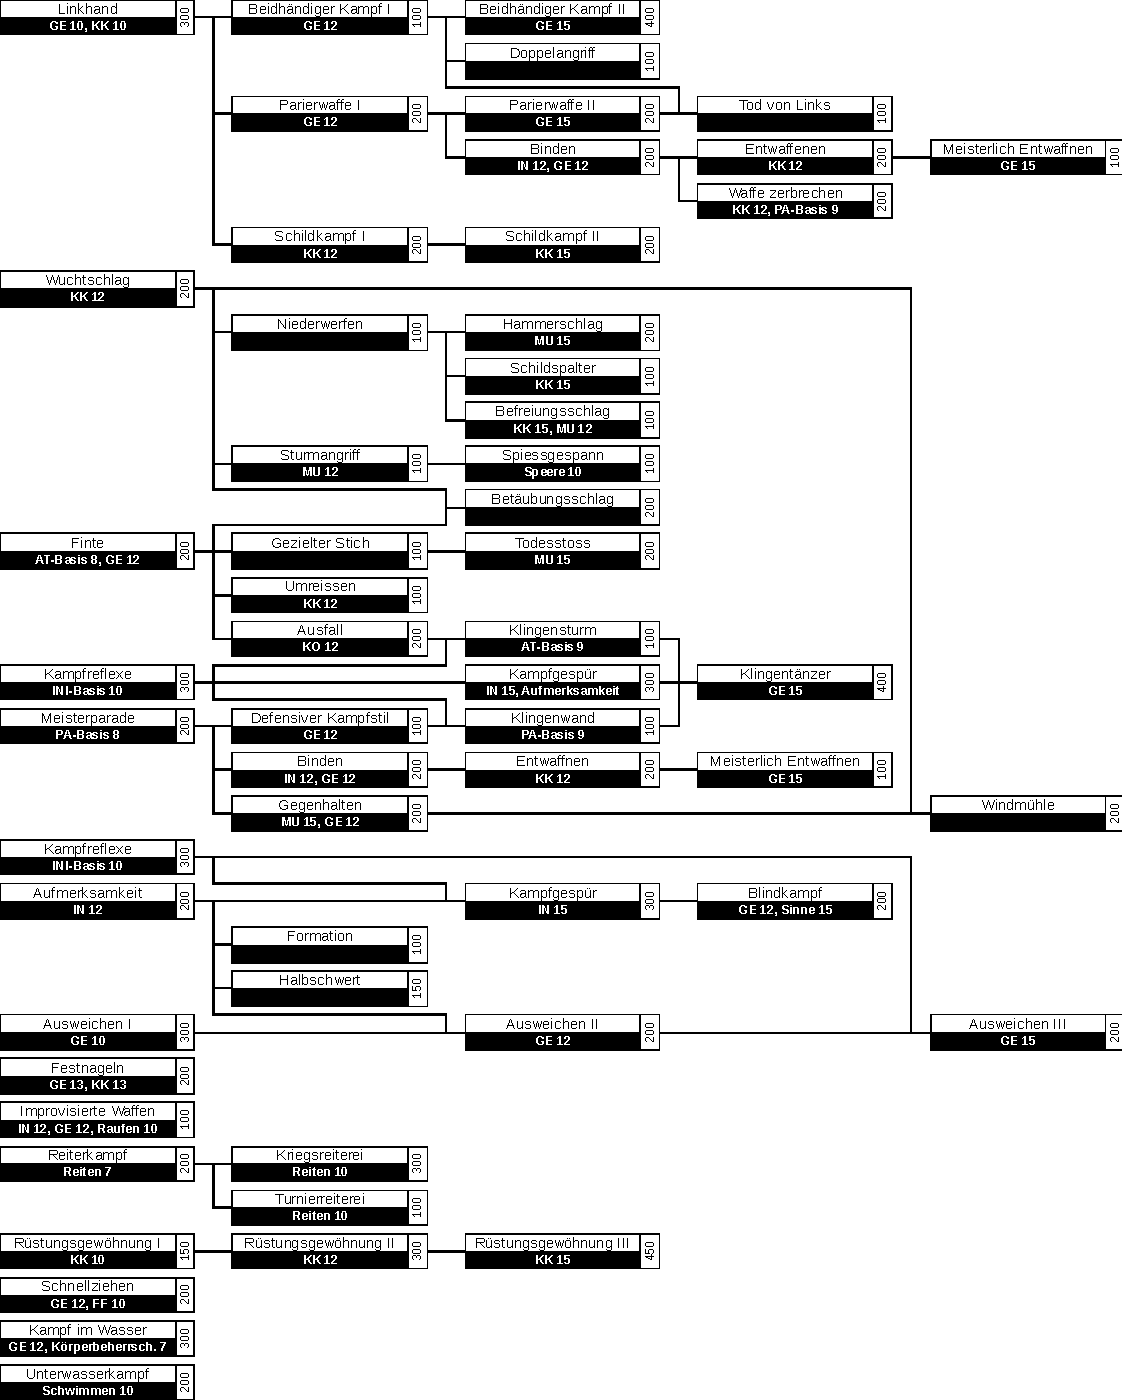
\includegraphics[width=16.986cm,height=21.179cm]{fig/bSF.pdf}
    \makebox[\textwidth][c]{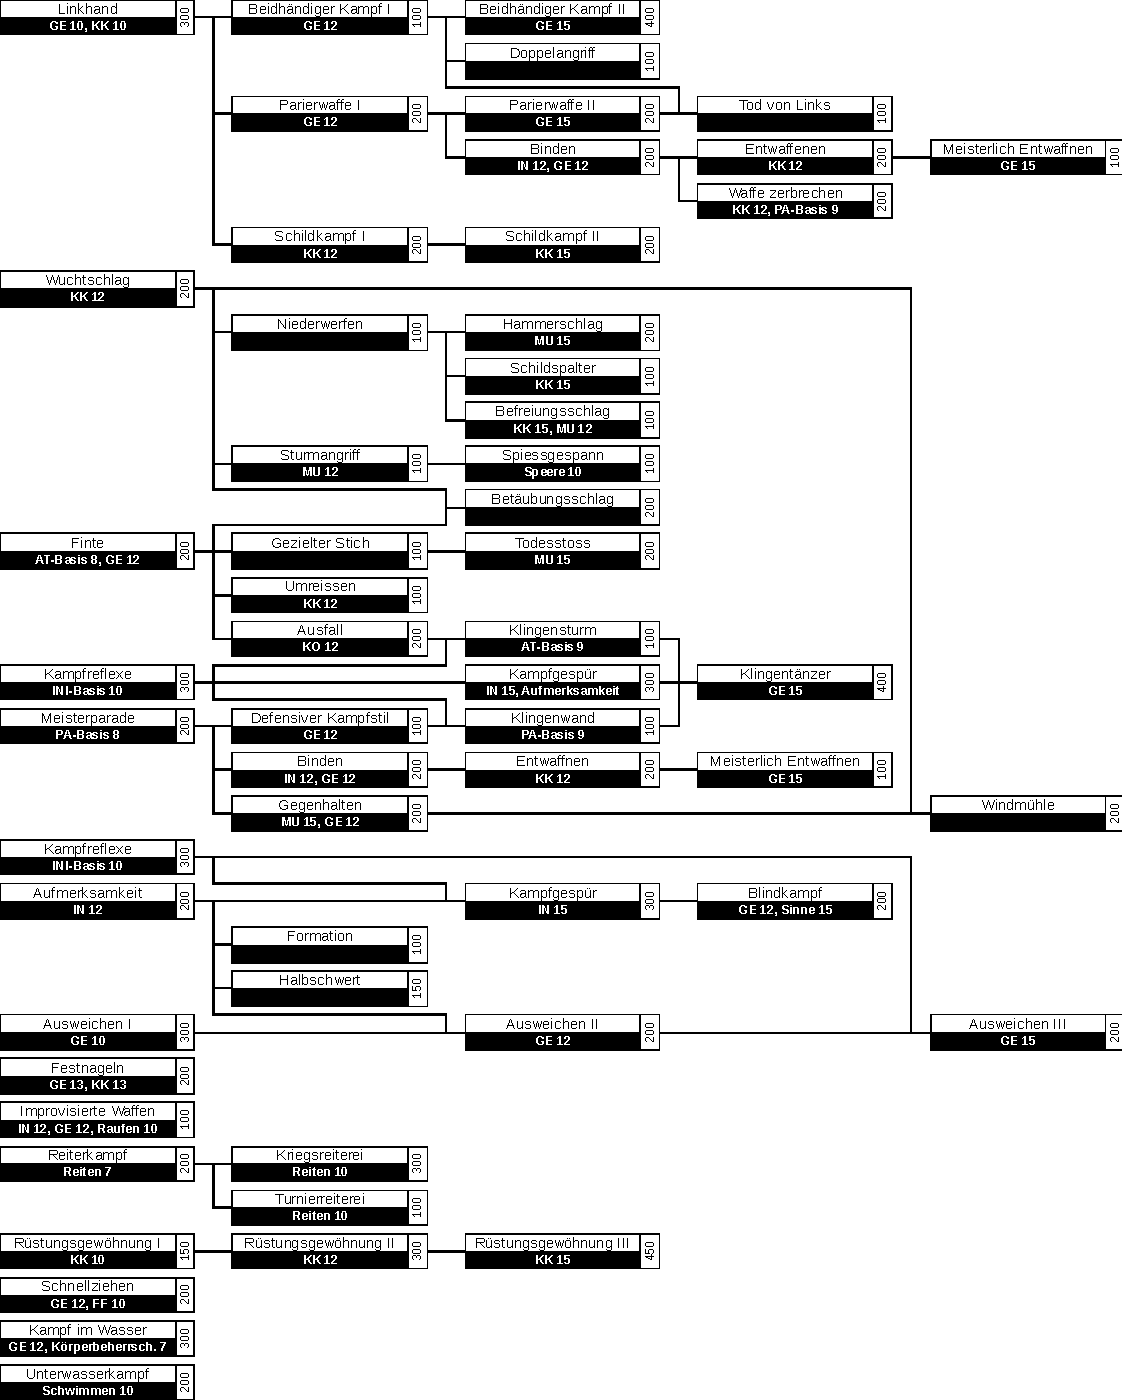
\includegraphics[width=16.986cm,height=21.179cm]{fig/bSF.pdf}}
    \caption{Übersicht der Sonderfertigkeiten für den bewaffneten Nahkampf}
    \label{fig.nSF}
\end{figure}

Abbildung \ref{fig.fSF} gibt eine Übersicht über alle Sonderfertigkeiten (mit AP-Kosten und Voraussetzungen), die im Fernkampf eingesetzt werden können.
Es handelt sich dabei nicht um die Manöver. Diese werden im Kapitel \ref{chap.fkM} beschrieben.

\begin{figure}
    \centering
    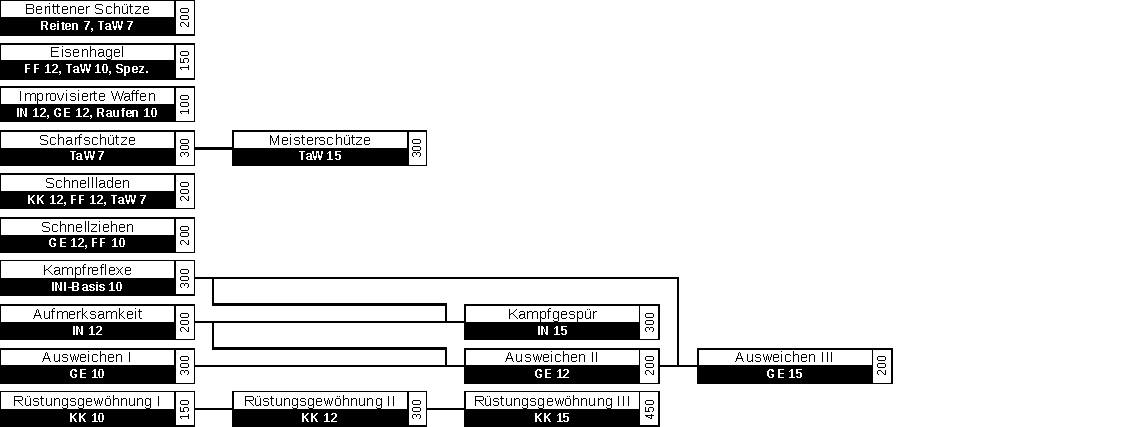
\includegraphics[width=16.93cm,height=6.454cm]{fig/fkSF.pdf}
    \caption{Übersicht der Sonderfertigkeiten für den Fernkampf}
    \label{fig.fSF}
\end{figure}

Abbildung \ref{fig.uSF} gibt eine Übersicht über alle Sonderfertigkeiten (mit AP-Kosten und Voraussetzungen), die im unbewaffneten Kampf eingesetzt werden können.
Es handelt sich dabei nicht um die Manöver.
Diese werden in den Kapiteln \ref{chap.uAT} und \ref{chap.uPA} beschrieben.
Hier gibt es einzelne Abweichungen zum DSA Regelwerk 4.1.

\begin{figure}
    \centering
    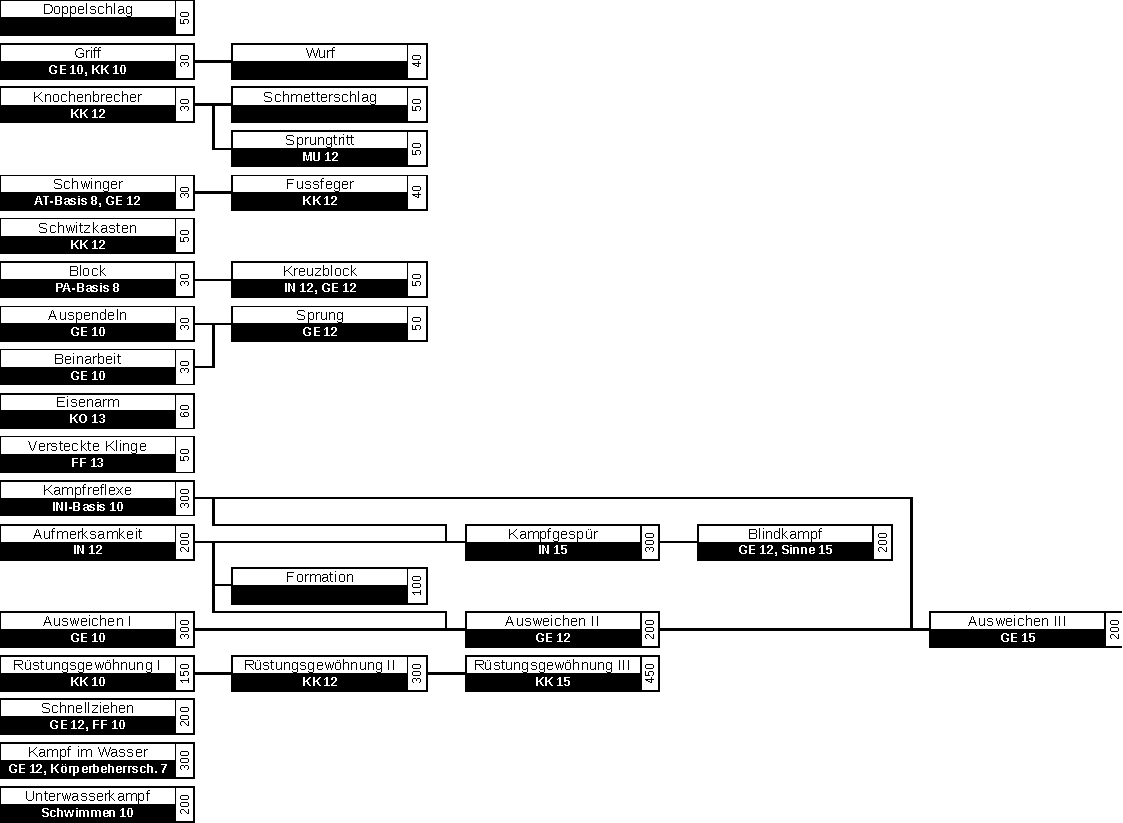
\includegraphics[width=16.976cm,height=12.437cm]{fig/uSF.pdf}
    \caption{Übersicht der Sonderfertigkeiten für den unbewaffneten Nahkampf}
    \label{fig.uSF}
\end{figure}

\subsection{Aufmerksamkeit}
\label{sf.aufmerksamkeit}
Gegen einen Kämpfer mit der SF \textStyleSF{\nameref{sf.aufmerksamkeit}} sind Passierschläge um 4 Punkte erschwert.
Ausserdem ist die IN-Probe um einen Hinterhalt oder eine Überraschung zu entdecken um 4 Punkte erleichtert.
\begin{description}
    \item[Voraussetzung]:
        IN 12
    \item [Kosten]:
        200 AP
    \item [Referenz]:
        WDS 73
\end{description}

\section{Ausfall}
\label{sf.ausfall}
Ermöglicht das Manöver \textStyleM{\nameref{aktion.ausfall}}.
\begin{description}
    \item[Voraussetzung:]
        KO 12, SF \textStyleSF{\nameref{sf.finte}}
    \item [Kosten:]
        200 AP
    \item [Referenz:]
        WDS 73
\end{description}

\section{Auspendeln}
\label{sf.auspendeln}
\textStyleAT{(Raufen oder Ringen)}
Mit der SF \textStyleSF{\nameref{sf.auspendeln}} ist der Verteidiger in der Lage, seinen Oberkörper scheinbar unabhängig von seinen Beinen zu bewegen.
Dies ist eine passive Sonderfertigkeit und erhöht den WM im Kampf gegen Unbewaffnete um 0/+1.
\begin{description}
    \item[Voraussetzung:]
        GE 10
    \item [Kosten:]
        30 AP
    \item [Referenz:]
        WDS 90
\end{description}

\subsection{Ausweichen}
\label{sf.ausweichen}
Die SFs \textStyleSF{\nameref{sf.ausweichen} I}, \textStyleSF{\nameref{sf.ausweichen} II} und \textStyleSF{\nameref{sf.ausweichen} III} erhöhen den Ausweichen-Wert um je 3 Punkte.
Dieser Wert berechnet sich aus PA-Basiswert – BE + Boni aus den Sonderfertigkeiten.

Je nach Behinderung ist es möglich zusätzlich zu einer Parade auch noch Auszuweichen.
Siehe Kapitel \ref{chap.A.AW}

\begin{description}
    \item[Voraussetzung]:
        GE 10 / GE 12, SF \textStyleSF{\nameref{sf.ausweichen} I}, SF \textStyleSF{\nameref{sf.aufmerksamkeit}} / GE 15, SF \textStyleSF{\nameref{sf.ausweichen} II}, SF \textStyleSF{\nameref{sf.kampfreflexe}}
    \item [Kosten]:
        300 AP / 200 AP / 200 AP, jeweils verbilligt für Helden mit dem Vorteil \textStyleVT{Schlangenmensch}
    \item [Referenz]:
        WDS 73
\end{description}

\section{Befreiungsschlag}
\label{sf.befreiungsschlag}
Ermöglicht das Manöver \textStyleM{\nameref{aktion.befreiungsschlag}}.
\begin{description}
    \item[Voraussetzung:]
        KK 15, MU 12, SF \textStyleSF{\nameref{sf.niederwerfen}}
    \item [Kosten:]
        100 AP
    \item [Referenz:]
        WDS 73
\end{description}

\subsection{Beidhändiger Kampf}
\label{sf.beidhaendiger_kampf}
Mit der SF \textStyleSF{\nameref{sf.beidhaendiger_kampf} I} werden die Abzüge für den Kampf mit der falschen Hand auf -3 /-3 reduziert und erlaubt zusätzliche Manöver sowie die Nutzung des KK-Bonus auf die TP der Linken Hand.

Die SF \textStyleSF{\nameref{sf.beidhaendiger_kampf} II} erlaubt alle Abzüge für den Kampf mit der falsch Hand zu ignorieren und stellt eine zusätzlich Angriffs- oder Abwehr-Aktion zur Verfügung.

Die Regelung bezüglich der Anzahl Aktionen pro Kampfrunde ist im Kapitel \ref{chap.aktion.beidhaendiger_kampf} beschrieben.

\begin{description}
    \item[Voraussetzung]:
        GE 12, SF \textStyleSF{\nameref{sf.linkhand}} / GE 15, SF \textStyleSF{\nameref{sf.beidhaendiger_kampf} I}
    \item [Kosten]:
        100 AP (50 AP mit Vorteil \textStyleVT{Beidhändig}, 75 AP mit Vorteil \textStyleVT{Linkshändig}) / 400 AP (200 AP mit Vorteil \textStyleVT{Beidhändig}, 300 AP mit Vorteil \textStyleVT{Linkshändig}, allfällige Kosten von \textStyleSF{\nameref{sf.tod_von_links}} können angerechnet werden)
    \item [Referenz]:
        WDS 73
\end{description}

\section{Beinarbeit}
\label{sf.beinarbeit}
\textStyleAT{(Raufen oder Ringen)}
Mit der SF \textStyleSF{\nameref{sf.beinarbeit}} ist der Verteidiger in der Lage auf sowohl sicheren wie auch beweglichen Stand zu achten.
Dies ist eine passive Sonderfertigkeit und erhöht den WM im Kampf gegen Unbewaffnete um 0/+1.
\begin{description}
    \item[Voraussetzung:]
        GE 10
    \item [Kosten:]
        30 AP
    \item [Referenz:]
        WDS 90
\end{description}

\section{Berittener Schütze}
\label{sf.berittener_schuetze}
Die SF \textStyleSF{\nameref{sf.berittener_schuetze}} erlaubt es einem Schützen die Waffe auf dem Reitpferd ohne zusätzlichen Zeitaufwand zu spannen.
Alle Aufschlage, mit denen ein Schuss oder Wurf vom sich bewegenden Reittier aus belegt sind, können halbiert werden. 
Vor dem Schuss oder Wurf muss keine Reiten-Probe abgelegt werden.
\begin{description}
    \item[Voraussetzung:]
        TaW \textStyleAT{Reiten} 7, TaW \textStyleAT{Fernkampftalent} 7
    \item [Kosten:]
        200 AP
    \item [Referenz:]
        WDS 95
\end{description}

\section{Betäubungsschlag}
\label{sf.betaeubungsschlag}
Ermöglicht das Manöver \textStyleM{\nameref{aktion.betaeubungsschlag}}.
\begin{description}
    \item[Voraussetzung:]
        SF \textStyleSF{\nameref{sf.finte}}, SF \textStyleSF{\nameref{sf.wuchtschlag}}
    \item [Kosten:]
        200 AP
    \item [Referenz:]
        WDS 73
\end{description}

\section{Binden}
\label{sf.binden}
Ermöglicht das Manöver \textStyleM{\nameref{bPA.binden}}.
\begin{description}
    \item[Voraussetzung:]
        IN 12, GE 12, SF \textStyleSF{\nameref{sf.meisterparade}} oder SF \textStyleSF{\nameref{sf.parierwaffen} I}
    \item [Kosten:]
        200 AP
    \item [Referenz:]
        WDS 73
\end{description}

\section{Blindkampf}
\label{sf.blindkampf}
Mit der SF \textStyleSF{\nameref{sf.blindkampf}} betragen die Abzüge auf AT / PA bei schlechter oder gar keiner Sicht maximal -2 / -2.
Ausserdem ist die IN-Probe um einen Hinterhalt oder eine Überraschung zu entdecken um weitere 2 Punkte erleichtert.
Diese SF gilt nicht für Fernkampffertigkeiten.

\begin{description}
    \item[Voraussetzung:]
        GE 12, TaW \textStyleTa{Sinnenschärfe} 15, SF \textStyleSF{\nameref{sf.kampfgespuer}}
    \item [Kosten:]
        200 AP
    \item [Referenz:]
        WDS 73
\end{description}

\section{Block}
\label{sf.block}
Ermöglicht das Manöver \textStyleM{\nameref{uPA.block}}.
\begin{description}
    \item[Voraussetzung:]
        PA-Basis 8
    \item [Kosten:]
        30 AP
    \item [Referenz:]
        WDS 91
\end{description}

\subsection{Defensiver Kampfstil}
\label{sf.defensiver_kampfstil}
Ermöglicht das Manöver \textStyleM{\nameref{aktion.defensiver_kampfstil}}.
\begin{description}
    \item[Voraussetzung]:
        GE 12, SF \textStyleSF{\nameref{sf.meisterparade}}
    \item [Kosten]:
        100 AP
    \item [Referenz]:
        WDS 73
\end{description}

\section{Doppelangriff}
\label{sf.doppelangriff}
Ermöglicht das Manöver \textStyleM{\nameref{aktion.doppelangriff}}.
\begin{description}
    \item[Voraussetzung:]
        SF \textStyleSF{\nameref{sf.beidhaendiger_kampf} I}
    \item [Kosten:]
        100 AP (75 AP für Helden mit dem Vorteil \textStyleVT{Beidhändig})
    \item [Referenz:]
        WDS 74
\end{description}

\section{Doppelschlag}
\label{sf.doppelschlag}
Ermöglicht das Manöver \textStyleM{\nameref{uAT.doppelschlag}}.
\begin{description}
    \item[Voraussetzung:]
        keine
    \item [Kosten:]
        50 AP
    \item [Referenz:]
        WDS 91
\end{description}

\section{Eisenarm}
\label{sf.eisenarm}
\textStyleAT{(Raufen oder Ringen)}
Mit der SF \textStyleSF{\nameref{sf.eisenarm}} erleidet der Verteidiger bei einer gelungen Parade gegen einen Bewaffneten nur TP(A).
Er ist zudem in der Lage gegen Bewaffnete das Manöver \textStyleM{\nameref{bPA.binden}} und \textStyleM{\nameref{bPA.entwaffnen}} einzusetzen (wenn er die entsprechende SF besitzt).
Ein Kämpfer mit Eisenarm erleidet keine Abzüge auf seinen INI-Modifikator im Kampf gegen Bewaffnete.
\begin{description}
    \item[Voraussetzung:]
        KO 13
    \item [Kosten:]
        60 AP
    \item [Referenz:]
        WDS 91
\end{description}

\section{Eisenhagel}
\label{sf.eisenhagel}
Ermöglicht das Manöver \textStyleM{\nameref{fkM.eisenhagel}}.
\begin{description}
    \item[Voraussetzung:]
        FF 12, TaW \textStyleTa{Wurfmesser} 10, entsprechnde Waffenspezialisierung
    \item [Kosten:]
        150 AP
    \item [Referenz:]
        WDS 95
\end{description}

\section{Entwaffnen}
\label{sf.entwaffnen}
Ermöglicht das Manöver \textStyleM{\nameref{bAT.entwaffnen}} aus der AT und \textStyleM{\nameref{bPA.entwaffnen}} aus der PA.
\begin{description}
    \item[Voraussetzung:]
        KK 12, SF \textStyleSF{\nameref{sf.binden}}
    \item [Kosten:]
        200 AP
    \item [Referenz:]
        WDS 74
\end{description}

\section{Festnageln}
\label{sf.festnageln}
Ermöglicht das Manöver \textStyleM{\nameref{aktion.festnageln}}.
\begin{description}
    \item[Voraussetzung:]
        GE 13, KK 13
    \item [Kosten:]
        200 AP
    \item [Referenz:]
        WDS 74
\end{description}

\section{Finte}
\label{sf.finte}
Erleichtert das Manöver \textStyleM{\nameref{aktion.finte}}.
\begin{description}
    \item[Voraussetzung:]
        GE 12, AT-Basis 8
    \item [Kosten:]
        200 AP
    \item [Referenz:]
        WDS 74
\end{description}

\section{Formation}
\label{sf.formation}
Ermöglicht das Manöver \textStyleM{\nameref{reaktion.formation}}.
\begin{description}
    \item[Voraussetzung:]
        SF \textStyleSF{\nameref{sf.aufmerksamkeit}}
    \item [Kosten:]
        100 AP
    \item [Referenz:]
        WDS 74
\end{description}

\section{Fussfeger}
\label{sf.fussfeger}
Ermöglicht das Manöver \textStyleM{\nameref{uAT.fussfeger}}.
\begin{description}
    \item[Voraussetzung:]
        KK 12, SF \textStyleSF{\nameref{sf.schwinger}}
    \item [Kosten:]
        40 AP
    \item [Referenz:]
        WDS 91
\end{description}

\subsection{Gegenhalten}
\label{sf.gegenhalten}
Ermöglicht das Manöver \textStyleM{\nameref{aktion.gegenhalten}}.
\begin{description}
    \item[Voraussetzung]:
        MU 15, GE 12, SF \textStyleSF{\nameref{sf.meisterparade}}
    \item [Kosten]:
        200 AP
    \item [Referenz]:
        WDS 74
\end{description}

\section{Gezielter Stich}
\label{sf.gezielter_stich}
Ermöglicht das Manöver \textStyleM{\nameref{aktion.gezielter_stich}}.
\begin{description}
    \item[Voraussetzung:]
        SF \textStyleSF{\nameref{sf.finte}}
    \item [Kosten:]
        100 AP
    \item [Referenz:]
        WDS 74
\end{description}

\section{Griff}
\label{sf.griff}
Ermöglicht das Manöver \textStyleM{\nameref{uAT.griff}}.
\begin{description}
    \item[Voraussetzung:]
        GE 10, KK 10
    \item [Kosten:]
        30 AP
    \item [Referenz:]
        WDS 91
\end{description}

\section{Halbschwert}
\label{sf.halbschwert}
Ein Kämpfer mit der SF \textStyleSF{\nameref{sf.halbschwert}} kann auch Parieren wenn er \textStyleM{\nameref{aktion.unterlaufen}} wurde.
\begin{description}
    \item[Voraussetzung:]
        SF \textStyleSF{\nameref{sf.aufmerksamkeit}}
    \item [Kosten:]
        150 AP
    \item [Referenz:]
        WDS 74
\end{description}

\subsection{Hammerschlag}
\label{sf.hammerschlag}
Ermöglicht das Manöver \textStyleM{\nameref{aktion.hammerschlag}}.
\begin{description}
    \item[Voraussetzung]:
        MU 15, SF \textStyleSF{\nameref{sf.niederwerfen}}
    \item [Kosten]:
        200 AP
    \item [Referenz]:
        WDS 74
\end{description}

\subsection{Improvisierte Waffen}
\label{sf.improvisierte_waffen}
Ein Kenner der SF \textStyleSF{\nameref{sf.improvisierte_waffen}} kann alle Mali im Kampf mit improvisierten Waffen ignorieren.
Die Waffen werden jedoch auch mit dieser SF nicht stabiler.

Nachfolgend die Mali für Kämpfer ohne Kenntnis dieser SF:

\begin{itemize}
    \item keine Manöver ausser Wuchtschlag (nur halbe Ansage als Schaden)
    \item Patzer auch bei 19, Prüfwurf um zusätzlich 5 erschwert
    \item Bruchfaktor Wurf bei jeder AT und PA
\end{itemize}

\begin{description}
    \item[Voraussetzung]:
        IN 12, TaW \textStyleTa{Raufen} 10, TaW \textStyleTa{Wurfwaffe} 10 wenn für Wurfwaffen verwendet
    \item [Kosten]:
        100 AP
    \item [Referenz]:
        WDS 74
\end{description}

\subsection{Kampf im Wasser}
\label{sf.kampf_im_wasser}
Mit der SF \textStyleSF{\nameref{sf.kampf_im_wasser}} werden alle Abzüge für den Kampf im Wasser halbiert.
\begin{description}
    \item[Voraussetzung]:
        GE 12, TaW \textStyleTa{Körperbeherrschung} 7
    \item [Kosten]:
        100 AP
    \item [Referenz]:
        WDS 74
\end{description}

\subsection{Kampfgespür}
\label{sf.kampfgespuer}
Die SF \textStyleSF{\nameref{sf.kampfgespuer}} bringt einen Bonus +2 auf den INI-Wert.
Gegen einen Kämpfer mit dieser SF ist ein Passierschlag um weitere 2 Punkte erschwert.
Ausserdem ist die IN-Probe um einen Hinterhalt oder eine Überraschung zu entdecken um weitere 4 Punkte erleichtert.
Weiter sind die Manöver \textStyleM{aktion.klingesturm} und \textStyleM{aktion.klingenwand} optimaler einsetzbar (Details siehe beim entsprechenden Manöver).

Der Einfluss der Initiative im Kampfgeschehen ist im Kapitel \ref{chap.INI} beschrieben.
\begin{description}
    \item[Voraussetzung]:
        IN 15, SF \textStyleSF{\nameref{sf.aufmerksamkeit}}, SF \textStyleSF{\nameref{sf.kampfreflexe}}
    \item [Kosten]:
        300 AP
    \item [Referenz]:
        WDS 74/75
\end{description}

\section{Kampfreflexe}
\label{sf.kampfreflexe}
Die SF \textStyleSF{\nameref{sf.kampfreflexe}} bringt einen Bonus +4 auf den INI-Wert.
Dieser Bonus kommt nur zum Tragen, bei BE kleiner oder gleich 4.

Der Einfluss der Initiative im Kampfgeschehen ist im Kapitel \ref{chap.ini} beschrieben.
\begin{description}
    \item[Voraussetzung:]
        INI-Basis 10
    \item [Kosten:]
        300 AP
    \item [Referenz:]
        WDS 75
\end{description}

\section{Klingensturm}
\label{sf.klingensturm}
Ermöglicht das Manöver \textStyleM{\nameref{bAT.klingensturm}}.
\begin{description}
    \item[Voraussetzung:]
        AT-Basis 9, SF \textStyleSF{\nameref{sf.ausfall}}, SF \textStyleSF{\nameref{sf.kampfreflexe}}
    \item [Kosten:]
        100 AP
    \item [Referenz:]
        WDS 75
\end{description}

\section{Klingentänzer}
\label{sf.klingentaenzer}
Die SF \textStyleSF{\nameref{sf.klingentaenzer}} bringt einen Bonus +4 auf den INI-Wert.
Ausserdem muss mit dieser SF eine allfällige negative Qualität nicht mehr vom Schaden abgezogen werden.
Weiter sind die Manöver \textStyleM{\nameref{bAT.klingensturm}} und \textStyleM{\nameref{bPA.klingenwand}} optimaler einsetzbar (Details siehe beim entsprechenden Manöver).

Der Einfluss der Initiative im Kampfgeschehen ist im Kapitel \ref{chap.ini} beschrieben.
\begin{description}
    \item[Voraussetzung:]
        GE 15, SF \textStyleSF{\nameref{sf.kampfgespuer}}, SF \textStyleSF{\nameref{sf.klingenwand}}, SF \textStyleSF{\nameref{sf.klingensturm}}
    \item [Kosten:]
        400 AP
    \item [Referenz:]
        WDS 75
\end{description}

\subsection{Klingenwand}
\label{sf.klingenwand}
Ermöglicht das Manöver \textStyleM{\nameref{reaktion.klingenwand}}.
\begin{description}
    \item[Voraussetzung]:
        PA-Basis 9, SF \textStyleSF{\nameref{sf.defensiver_kampfstil}}, SF \textStyleSF{\nameref{sf.kampfreflexe}}
    \item [Kosten]:
        100 AP
    \item [Referenz]:
        WDS 75
\end{description}

\section{Knochenbrecher}
\label{sf.knochenbrecher}
Erleichtert das Manöver \textStyleM{\nameref{uAT.knochenbrecher}}.
\begin{description}
    \item[Voraussetzung:]
        KK 12
    \item [Kosten:]
        30 AP
    \item [Referenz:]
        WDS 91 (Gerade, Handkante, Knie, Kopfstoss), WDS 92 (Tritt)
\end{description}

\section{Kreuzblock}
\label{sf.kreuzblock}
Ermöglicht das Manöver \textStyleM{\nameref{uPA.kreuzblock}}.
\begin{description}
    \item[Voraussetzung:]
        IN 12, GE 12, SF \textStyleSF{\nameref{sf.block}}
    \item [Kosten:]
        50 AP
    \item [Referenz:]
        WDS 91
\end{description}

\section{Kriegsreiterei}
\label{sf.kriegsreiterei}
Reiter mit der SF \textStyleSF{\nameref{sf.kriegsreiterei}} müssen nur ein Viertel der Zuschläge hinnehmen, mit denen die Reiten Proben im Kampf belegt sind (Ausgenommen sind die Erschwernisse aus einem angesagten Lanzenangriff).
Das Pferd eines Kriegsreiters erhält \ 3 Punkte Erleichterung auf seine Paraden.
\begin{description}
    \item[Voraussetzung:]
        TaW \textStyleTa{Reiten} 10, SF \textStyleSF{\nameref{sf.reiterkampf}}
    \item [Kosten:]
        300 AP
    \item [Referenz:]
        WDS 101
\end{description}

\subsection{Linkhand}
\label{sf.linkhand}
Die SF \textStyleSF{\nameref{sf.linkhand}} vermindert die Abzüge für den Kampf mit der falschen Hand auf -6 / -6 und gibt einem Schildkämpfer einen Bonuspunkt auf den PA-Wert.
\begin{description}
    \item[Voraussetzung]:
        KK 10, GE 10
    \item [Kosten]:
        300 AP
    \item [Referenz]:
        WDS 75
\end{description}

\section{Meisterliches Entwaffnen}
\label{sf.meisterliches_entwaffnen}
Die SF erlaubt das Manöver \textStyleM{\nameref{bAT.entwaffnen}} auch auf Kämpfer mit einer Zweihandwaffe.
\begin{description}
    \item[Voraussetzung:]
        GE 15, SF \textStyleSF{\nameref{sf.entwaffnen}}
    \item [Kosten:]
        100 AP
    \item [Referenz:]
        WDS 75
\end{description}

\subsection{Meisterparade}
\label{sf.meisterparade}
Ermöglicht das Manöver \textStyleM{\nameref{aktion.meisterparade}}.
\begin{description}
    \item[Voraussetzung]:
        PA-Basis 8
    \item [Kosten]:
        200 AP
    \item [Referenz]:
        WDS 75
\end{description}

\subsection{Meisterschütze}
\label{sf.meisterschuetze}
Mit der SF \textStyleSF{\nameref{sf.meisterschuetze}} erleidet der Schütze / Werfer keinen Aufschlag für einen \textStyleM{\nameref{fernkampf.schnellschuss}} (ohne SF 2 Aktionen).
Beim Manöver \textStyleM{\nameref{fernkampf.ansage}} kann eine maximale Ansage in Höhe seines Fernkampfwerts (anstelle nur seines Talentwerts) machen und es muss nur eine zusätzliche Aktion aufgewendet werden.
Ein \textStyleSF{\nameref{sf.meisterschuetze}} ignoriert Zuschläge aus Seitenwind und Steilschüssen.
\begin{description}
    \item[Voraussetzung]:
        TaW \textStyleTa{Fernkampftalent} 15, SF \textStyleSF{\nameref{sf.scharfschuetze}}, muss für jedes Fernkampftalent separat erlernt werden
    \item [Kosten]:
        300 AP
    \item [Referenz]:
        WDS 95
\end{description}

\subsection{Niederwerfen}
\label{sf.niederwerfen}
Ermöglicht das Manöver \textStyleM{\nameref{aktion.niederwerfen}}.
\begin{description}
    \item[Voraussetzung]:
        SF \textStyleSF{\nameref{sf.wuchtschlag}}
    \item [Kosten]:
        100 AP
    \item [Referenz]:
        WDS 75
\end{description}

\subsection{Parierwaffen}
\label{sf.parierwaffen}
Mit der SF \textStyleSF{\nameref{sf.parierwaffen} I} kann der Kämpfer eine Parierwaffe mit dem Parade-Wert der Hauptwaffe -1 + PA-WM der Parierwaffe verwenden.

Mit der SF \textStyleSF{\nameref{sf.parierwaffen} II} kann der Kämpfer eine Parierwaffe mit dem Parade-Wert der Hauptwaffe +2 + PA-WM der Parierwaffe verwenden und erhält ausserdem eine zusätzliche Reaktion.

Die Regelung bezüglich der Anzahl Aktionen pro Kampfrunde ist im Kapitel \ref{chap.aktion.parierwaffen} beschrieben.
\begin{description}
    \item[Voraussetzung]:
        GE 12, SF \textStyleSF{\nameref{sf.linkhand}} / GE 15, SF \textStyleSF{\nameref{sf.parierwaffen} I}
    \item [Kosten]:
        200 AP (150 AP für Helden mit dem Vorteil \textStyleVT{Beidhändig}) / 200 AP (150 AP für Helden mit dem Vorteil \textStyleVT{Beidhändig})
    \item [Referenz]:
        WDS 75/76
\end{description}

\subsection{Reiterkampf}
\label{sf.reiterkampf}
Reiter mit der SF \textStyleSF{\nameref{sf.reiterkampf}} müssen nur die Hälfte der Zuschläge hinnehmen, mit denen die Reiten Proben im Kampf belegt sind (Ausgenommen sind die Erschwernisse aus einem angesagten Lanzenangriff).
Ausserdem muss keine Probe gewürfelt werden um das Pferd an den Gegner heranzubringen oder einen Lanzenangriff zu beginnen (Ausgenommen ist der angesagte Lanzenangriff).
Im Kampf gegen Fuss Kämpfer sind alle Attacken um 3 erleichtert.
\begin{description}
    \item[Voraussetzung]:
        TaW \textStyleTa{Reiten} 7
    \item [Kosten]:
        200 AP
    \item [Referenz]:
        WDS 101
\end{description}

\subsection{Rüstungsgewöhnung}
\label{sf.ruestungsgewoehnung}
Mit der SF \textStyleSF{\nameref{sf.ruestungsgewoehnung} I} sinkt die BE eines bestimmten Rüstungstyps um einen Punkt.

Mit der SF \textStyleSF{\nameref{sf.ruestungsgewoehnung} II} sinkt die BE aller Rüstungen um einen Punkt.

Mit der SF \textStyleSF{\nameref{sf.ruestungsgewoehnung} III} sinkt die BE aller Rüstungen um zwei Punkte.
Ausserdem wird nur die Hälfte der Behinderung vom INI-Wert abgezogen.

Der Einfluss der Initiative im Kampfgeschehen ist im Kapitel \ref{chap.INI} beschrieben.
\begin{description}
    \item[Voraussetzung]:
        KK 10 / KK 12, SF \textStyleSF{\nameref{sf.ruestungsgewoehnung} I} / KK 15, SF \textStyleSF{\nameref{sf.ruestungsgewoehnung} II}
    \item [Kosten]:
        150 AP (225 AP für Helden mit dem Vorteil \textStyleVT{Akademische Ausbildung (Magier)}) / 300 AP (450 AP für Helden mit dem Vorteil \textStyleVT{Akademische Ausbildung (Magier)}) / 450 AP (675 AP für Helden mit dem Vorteil \textStyleVT{Akademische Ausbildung (Magier)})
    \item [Referenz]:
        WDS 76
\end{description}

\section{Scharfschütze}
\label{sf.scharfschuetze}
Mit der SF \textStyleSF{\nameref{sf.scharfschuetze}} erleidet der Schütze / Werfer nur einen Aufschlag von 1 Aktion (anstelle von 2 Aktionen) für einen \textStyleM{\nameref{fkM.schnellschuss}}.
Beim Manöver \textStyleM{\nameref{fkM.ansage}}, kann die volle Ansage zu den TP addiert werden und es werden zwei Aktionen weniger zum Zielen benötigt (mindestens aber eine zusätzliche Aktion).
Scharfschützen benötigen beim Manöver \textStyleM{\nameref{fkM.zielen}} eine Aktion pro Punkt reduzierte Erschwernis.
\begin{description}
    \item[Voraussetzung:]
        TaW \textStyleTa{Fernkampftalent} 7, muss für jedes Fernkampftalent separat erlernt werden
    \item [Kosten:]
        300 AP
    \item [Referenz:]
        WDS 95
\end{description}

\section{Schildkampf}
\label{sf.schildkampf}
Die SF \textStyleSF{\nameref{sf.schildkampf} I} gibt einem Schildkämpfer 2 weitere zusätzlich Punkte auf seinen Parade-Basiswert.

Die SF \textStyleSF{\nameref{sf.schildkampf} II} gibt einem Schildkämpfer 2 weitere zusätzlich Punkte auf seinen Parade-Basiswert.
Zudem erhält der Schildkämpfer eine zusätzliche Reaktion.

Die Regelung bezüglich der Anzahl Aktionen pro Kampfrunde ist im Kapitel \ref{chap.aktion.schildkampf} beschrieben.
\begin{description}
    \item[Voraussetzung:]
        KK 12, SF \textStyleSF{\nameref{sf.linkhand}} / KK 15, SF \textStyleSF{\nameref{sf.schildkampf} I}
    \item [Kosten:]
        200 AP (150 AP für Helden mit dem Vorteil \textStyleVT{Beidhändig}) / 200 AP (150 AP für Helden mit dem Vorteil \textStyleVT{Beidhändig})
    \item [Referenz:]
        WDS 76
\end{description}

\section{Schildspalter}
\label{sf.schildspalter}
Ermöglicht das Manöver \textStyleM{\nameref{bAT.schildspalter}}.
\begin{description}
    \item[Voraussetzung:]
        KL 15, SF \textStyleSF{\nameref{sf.niederwerfen}}
    \item [Kosten:]
        100 AP
    \item [Referenz:]
        WDS 76
\end{description}

\section{Schmetterschlag}
\label{sf.schmetterschlag}
Ermöglicht das Manöver \textStyleM{\nameref{uAT.schmetterschlag}}.
\begin{description}
    \item[Voraussetzung:]
        SF \textStyleSF{\nameref{sf.knochenbrecher}}
    \item [Kosten:]
        50 AP
    \item [Referenz:]
        WDS 92
\end{description}

\section{Schnellladen}
\label{sf.schnellladen}
Die SF \textStyleSF{\nameref{sf.schnellladen}} reduziert die Ladezeiten für Bögen um eine Aktion (betragen aber mindestens 1 Aktion).
Die SF kann auch für Armbrüste erlernt werden: Es werden nur noch drei Viertel der angegebenen Ladezeiten benötigt.
Diese SF kann nur eingesetzt werden, wenn die BE des Kämpfers 4 oder weniger beträgt.
\begin{description}
    \item[Voraussetzung:]
        FF 12, KK12, TaW \textStyleTa{Armbrust/Bogen} 7, muss für jedes Fernkampftalent separat erlernt werden
    \item [Kosten:]
        200 AP
    \item [Referenz:]
        WDS 95
\end{description}

\section{Schnellziehen}
\label{sf.schnellziehen}
Mit der SF \textStyleSF{\nameref{sf.schnellziehen}} können Waffen aus einer Gürtelscheide in einer freien Aktion (sonst eine Aktion), Waffen vom Rücken in einer Aktion (sonst zwei Aktionen) und Schilde vom Rücken in drei Aktionen (sonst fünf Aktionen) gezogen werden.
Dies ist nur möglich \ bei BE kleiner oder gleich 4.
\begin{description}
    \item[Voraussetzung:]
        GE 12, FF 10
    \item [Kosten:]
        200 AP (100 AP für Helden mit dem Vorteil \textStyleVT{Schlangenmensch})
    \item [Referenz:]
        WDS 76/95
\end{description}

\section{Schwinger}
\label{sf.schwinger}
Erleichtert das Manöver \textStyleM{\nameref{uAT.schwinger}}.
\begin{description}
    \item[Voraussetzung:]
        GE 12, AT-Basis 8
    \item [Kosten:]
        30 AP
    \item [Referenz:]
        WDS 92
\end{description}

\section{Schwitzkasten}
\label{sf.schwitzkasten}
Ermöglicht das Manöver \textStyleM{\nameref{uAT.schwitzkasten}}.
\begin{description}
    \item[Voraussetzung:]
        KK 12
    \item [Kosten:]
        50 AP
    \item [Referenz:]
        WDS 92, WDS 92 (Würgegriff)
\end{description}

\section{Spiessgespann}
\label{sf.spiessgespann}
Mit der SF \textStyleSF{\nameref{sf.spiessgespann}} kann ein überlanger Spiess (Pike, Drachentöter) gleichzeitig von zwei Personen geführt werden.
Wenn beiden Kämpfer die AT (positive Qualität) gelingt, so richtet ein \textStyleSF{\nameref{sf.spiessgespann}} doppelten Schaden an.
Zudem können die beiden Kämpfer ihre KK addieren und mit der TP/KK der Waffe verrechnen.
Die Qualität des Angriffs entspricht der niedrigsten Qualität der beiden Kämpfer.
Ist die Qualität negativ, wird der Schaden nicht verdoppelt und die höchste negative Qualität wird vom Schaden abgezogen.
Die Initiative des Spiessgespanns ist so hoch wie die niedrigste INI der beiden Kämpfer.
Es können nur Manöver eingesetzt werden, die beide Kämpfer beherrschen.
\begin{description}
    \item[Voraussetzung:]
        TaW \textStyleTa{Speere} 10, SF \textStyleSF{\nameref{sf.sturmangriff}}
    \item [Kosten:]
        100 AP
    \item [Referenz:]
        WDS 76
\end{description}

\section{Sprung}
\label{sf.sprung}
Ermöglicht das Manöver \textStyleM{\nameref{uPA.sprung}}.
\begin{description}
    \item[Voraussetzung:]
        GE 12, SF \textStyleSF{\nameref{sf.auspendeln}}, SF \textStyleSF{\nameref{sf.beinarbeit}}
    \item [Kosten:]
        50 AP
    \item [Referenz:]
        WDS 92
\end{description}

\section{Sprungtritt}
\label{sf.sprungtritt}
Ermöglicht das Manöver \textStyleM{\nameref{uAT.sprungtritt}}.
\begin{description}
    \item[Voraussetzung:]
        MU 12, \textStyleSF{\nameref{sf.knochenbrecher}}
    \item [Kosten:]
        50 AP
    \item [Referenz:]
        WDS 92
\end{description}

\subsection{Sturmangriff}
\label{sf.sturmangriff}
Ermöglicht das Manöver \textStyleM{\nameref{aktion.sturmangriff}}.
\begin{description}
    \item[Voraussetzung]:
        MU 12, SF \textStyleSF{\nameref{sf.wuchtschlag}}
    \item [Kosten]:
        100 AP
    \item [Referenz]:
        WDS 76
\end{description}

\section{Tod von Links}
\label{sf.tod_von_links}
Ermöglicht das Manöver \textStyleM{\nameref{bAT.tod_von_links}}.
\begin{description}
    \item[Voraussetzung:]
        SF \textStyleSF{\nameref{sf.beidhaendiger_kampf} I}, SF \textStyleSF{\nameref{sf.parierwaffen} II}
    \item [Kosten:]
        100 AP (75 AP für Helden mit dem Vorteil \textStyleVT{Beidhändig})
    \item [Referenz:]
        WDS 77
\end{description}

\section{Todesstoss}
\label{sf.todesstoss}
Ermöglicht das Manöver \textStyleM{\nameref{aktion.todesstoss}}.
\begin{description}
    \item[Voraussetzung:]
        MU 15, SF \textStyleSF{\nameref{sf.gezielter_stich}}
    \item [Kosten:]
        200 AP
    \item [Referenz:]
        WDS 77
\end{description}

\section{Turnierreiterei}
\label{sf.turnierreiterei}
Mit der SF \textStyleSF{\nameref{sf.turnierreiterei}} sind alle Lanzenreiten Proben um 5 Punkte erleichtert und die Reiten-Probe um nach einem Treffer im Turnier im Sattel zu bleiben ist nur um die Hälfte der Zuschläge erschwert.
\begin{description}
    \item[Voraussetzung:]
        TaW \textStyleAT{Reiten} 10, SF \textStyleSF{\nameref{sf.reiterkampf}}
    \item [Kosten:]
        100 AP
    \item [Referenz:]
        WDS 101
\end{description}

\section{Umreissen}
\label{sf.umreissen}
Ermöglicht das Manöver \textStyleM{\nameref{aktion.umreissen}}.
\begin{description}
    \item[Voraussetzung:]
        KK 12, SF \textStyleSF{\nameref{sf.finte}}
    \item [Kosten:]
        100 AP
    \item [Referenz:]
        WDS 77
\end{description}

\subsection{Unterwasserkampf}
\label{sf.unterwasserkampf}
Mit der SF \textStyleSF{\nameref{sf.unterwasserkampf}} entfallen die üblichen Abzüge auf AT / PA von -6 / -6 für den Kampf unter Wasser.
\begin{description}
    \item[Voraussetzung]:
        Taw \textStyleTa{Schwimmen} 10
    \item [Kosten]:
        200 AP
    \item [Referenz]:
        WDS 77
\end{description}

\section{Versteckte Klinge}
\label{sf.versteckte_klinge}
\textStyleAT{(Raufen)}
Mit der SF \textStyleSF{\nameref{sf.versteckte_klinge}} ist der Kämpfer ist in der Lage, eine Waffe mit der Distanzklasse Handgemenge mit seinen Raufen Kampfwerten einzusetzen.
\begin{description}
    \item[Voraussetzung:]
        FF 13
    \item [Kosten:]
        50 AP
    \item [Referenz:]
        WDS 92
\end{description}


\section{Waffe Zerbrechen}
\label{sf.waffe_zerbrechen}
Ermöglicht das Manöver \textStyleM{\nameref{bPA.waffe_zerbrechen}}
\begin{description}
    \item[Voraussetzung:]
        KK 12, PA-Basis 9, SF \textStyleSF{\nameref{sf.binden}}
    \item [Kosten:]
        200 AP
    \item [Referenz:]
        WDS 77
\end{description}

\section{Windmühle}
\label{sf.windmuehle}
Ermöglicht das Manöver \textStyleM{\nameref{bPA.windmuehle}}
\begin{description}
    \item[Voraussetzung:]
        SF \textStyleSF{\nameref{sf.gegenhalten}}, SF \textStyleSF{\nameref{sf.wuchtschlag}}
    \item [Kosten:]
        200 AP
    \item [Referenz:]
        WDS 77
\end{description}

\section{Wuchtschlag}
\label{sf.wuchtschlag}
Erleichtert das Manöver \textStyleM{\nameref{aktion.wuchtschlag}}.
\begin{description}
    \item[Voraussetzung:]
        KK 12
    \item [Kosten:]
        200 AP
    \item [Referenz:]
        WDS 77
\end{description}

\section{Wurf}
\label{sf.wurf}
Mit der SF \textStyleSF{\nameref{sf.wurf}} ist der Kämpfer in der Lage, das Manöver \textStyleM{\nameref{uAT.niederschlagen}} effektiver auszuführen.
\begin{description}
    \item[Voraussetzung:]
        SF \textStyleSF{\nameref{sf.griff}}
    \item [Kosten:]
        40 AP
    \item [Referenz:]
        WDS 93
\end{description}


%% -*-mode: Latex-*-
% !TEX root = kampf.tex
% authors: simon maurer
%
% file: uSF.tex
% contents: main content of the document
% Sccs-Id: %W% %G%

%==============================================================================

\section[Sonderfertigkeiten für den unbewaffneten Kampf]{\color{black}
Sonderfertigkeiten für den unbewaffneten Kampf}
{\sffamily\color{black}
Folgende Abbildung gibt eine Übersicht über alle Sonderfertigkeiten (mit
AP-Kosten und Voraussetzungen), die im unbewaffneten Kampf eingesetzt
werden können. Es handelt sich dabei nicht um die Manöver. Diese werden
in den Kapiteln 9 und 10 beschrieben. Hier gibt es einzelne
Abweichungen zum DSA Regelwerk 4.1.}


\bigskip



\begin{figure}
\centering
\includegraphics[width=16.976cm,height=12.437cm]{a110101kampfregelnskizze-img2.pdf}
\end{figure}
{\sffamily\color{black}
In den folgenden Unterkapitel werden Sonderfertigkeiten beschrieben, die
nicht Voraussetzung für ein bestimmtes Manöver sind, sondern einen
direkten Einfluss auf den Kämpfer und seine Fähigkeiten haben. Es
werden jedoch nur noch jene SFs beschrieben, die nicht bereits im
Kapitel 5 aufgelistet wurden.}

\subsection[Auspendeln (Raufen oder Ringen)]{Auspendeln
\textstyleEndnoteSymbol{(Raufen oder Ringen)}}
{\sffamily\color{black}
Mit der SF \testStyleSF{Auspendeln} ist der Verteidige in der
Lage, seinen Oberkörper scheinbar unabhängig von seinen Beinen zu
bewegen. Dies ist eine passive Sonderfertigkeit und erhöht den WM im
Kampf gegen Unbewaffnete um 0/+1.}

\subsection[Beinarbeit (Raufen oder Ringen)]{Beinarbeit
\textstyleEndnoteSymbol{(Raufen oder Ringen)}}
{\sffamily\color{black}
Mit der SF \testStyleSF{Beinarbeit} ist der Verteidiger in der
Lage auf sowohl sicheren wie auch Beweglichen Stand zu achten. Dies ist
eine passive Sonderfertigkeit und erhöht den WM im Kampf gegen
Unbewaffnete um 0/+1.}

\subsection[Eisenarm (Raufen oder Ringen)]{Eisenarm
\textstyleEndnoteSymbol{(Raufen oder Ringen)}}
{\sffamily\color{black}
Mit der SF \testStyleSF{Eisenarm} erleidet der Verteidiger bei
einer gelungen Parade gegen einen Bewaffneten nur TP(A). Er ist zudem
in der Lage gegen Bewaffnete das Manöver \testStyleSF{Binden}
und \testStyleSF{Entwaffnen} einzusetzen (wenn er die
entsprechende SF besitzt). Ein Kämpfer mit Eisenarm erleidet keine
Abzüge auf seinen INI-Modifikator im Kampf gegen Bewaffnete.}

\subsection[Versteckte Klinge (Raufen)]{Versteckte Klinge
\textstyleEndnoteSymbol{(Raufen)}}
{\sffamily\color{black}
Mit der SF \testStyleSF{Versteckte Klinge} ist der Kämpfer ist
in der Lage, eine Waffe mit der Distanzklasse Handgemenge mit seinen
Raufen Kampfwerten einzusetzen.}

\subsection{Wurf}
{\sffamily\color{black}
Mit der SF \testStyleSF{Wurf} ist der Kämpfer in der Lage, das
Manöver Niederschlagen/-werfen effektiver auszuführen.}

%% -*-mode: Latex-*-
% !TEX root = kampf.tex
% authors: simon maurer
%
% file: uSpez.tex
% contents: Unbewaffnete Spezialisierungen
% Sccs-Id: %W% %G%

%==============================================================================


\chapter{Waffenloser Kampf}
\label{chap.uSpez}
Im waffenlosen Kampf gelten im Allgemeninen folgende Modifikatoren (einige Werte können durch Sonderfertigkeiten verbessert werden):

\begin{itemize}
    \item WM gegen Unbewaffnete: 0/-2 (Siehe \textStyleSF{\nameref{sf.beinarbeit}} und \textStyleSF{\nameref{sf.auspendeln}})
    \item WM gegen Bewaffnete: -1/-2
    \item Wundschwelle Gegner: +2 (Siehe \textStyleSF{\nameref{uSpez.hammerfaust}} und \textStyleSF{\nameref{uSpez.hruruzat}})
    \item INI gegen Bewaffnete: -2 (Siehe \textStyleSF{\nameref{sf.eisenarm}})
    \item PA gegen Bewaffnete, wenn PA gelungen: Halbe TP (Siehe \textStyleSF{\nameref{sf.eisenarm}})
    \item AT gegen Bewaffnete, wenn Gegner pariert: Halbe TP (nur Waffenschaden) (Siehe \textStyleSF{\nameref{sf.eisenarm}})
\end{itemize}

Der waffenlose Kampf erlaubt verschiedene Spezialisierungen, welche als Sonderfertigkeiten erworben werden können:

\section{Bornländisch}
\label{uSpez.bornlaendisch}
\begin{description}
    \item[Voraussetzung:]
        TaW Raufen 5, TaW Ringen 5
    \item[Kosten:]
        100 AP
    \item[Spezialisierung:]
        Ringen +1/+1
    \item[Verbilligte SFs:]
        \textStyleSF{\nameref{sf.auspendeln}}, \textStyleSF{\nameref{sf.block}}, \textStyleSF{\nameref{sf.fussfeger}}, \textStyleSF{\nameref{sf.griff}}, \textStyleSF{\nameref{sf.knochenbrecher}}, \textStyleSF{\nameref{sf.schwinger}}, \textStyleSF{\nameref{sf.schwitzkasten}}, \textStyleSF{\nameref{sf.wurf}}
    \item [Referenz:]
        WDS 89
\end{description}


\section{Gladiatorenstil}
\label{uSpez.gladiatorenstil}
\begin{description}
    \item[Voraussetzung:]
        TaW Raufen 7, TaW Ringen 7
    \item[Kosten:]
        150 AP
    \item[Spezialisierung:]
        Ringen oder Raufen +1/+1
    \item[Verbilligte SFs:]
        \textStyleSF{\nameref{sf.auspendeln}}, \textStyleSF{\nameref{sf.beinarbeit}}, \textStyleSF{\nameref{sf.block}}, \textStyleSF{\nameref{sf.doppelschlag}}, \textStyleSF{\nameref{sf.eisenarm}}, \textStyleSF{\nameref{sf.fussfeger}}, \textStyleSF{\nameref{sf.griff}}, \textStyleSF{\nameref{sf.knochenbrecher}}, \textStyleSF{\nameref{sf.kreuzblock}}, \textStyleSF{\nameref{sf.schwinger}}, \textStyleSF{\nameref{sf.sprung}}, \textStyleSF{\nameref{sf.sprungtritt}}, \textStyleSF{\nameref{sf.wurf}}, \textStyleSF{\nameref{sf.kreuzblock}}
    \item[Speziell:]
        Kann bis zu 3 Punkten weniger echten Schaden anrichten und stattdessen diese Punkte auf den Ausdauerschaden schlagen.
    \item [Referenz:]
        WDS 89
\end{description}

\section{Hammerfaust}
\label{uSpez.hammerfaust}
\begin{description}
    \item[Voraussetzung:]
        TaW Raufen 7
    \item[Kosten:]
        150 AP
    \item[Spezialisierung:]
        Raufen +1/+1
    \item[Verbilligte SFs:]
        \textStyleSF{\nameref{sf.auspendeln}}, \textStyleSF{\nameref{sf.block}}, \textStyleSF{\nameref{sf.doppelschlag}}, \textStyleSF{\nameref{sf.eisenarm}}, \textStyleSF{\nameref{sf.knochenbrecher}}, \textStyleSF{\nameref{sf.kreuzblock}}, \textStyleSF{\nameref{sf.schmetterschlag}}, \textStyleSF{\nameref{sf.schwinger}}
    \item[Wundschwelle Gegner:]
        0
    \item[Speziell:]
        Kann mit der blossen Faust massive Gegenstände beschädigen.
        TP(A) als Strukturschaden.
        Wenn der Kämpfer die SF Ausfall beherrscht kann, er dieses Manöver auch im waffenlosen Kampf anwenden.
    \item [Referenz:]
        WDS 89
\end{description}

\section{Hruruzat}
\label{uSpez.hruruzat}
\begin{description}
    \item[Voraussetzung:]
        TaW Raufen 10, TaW Ringen 7
    \item[Kosten:]
        200 AP
    \item[Spezialisierung:]
        Raufen +1/+1
    \item[Verbilligte SFs:]
        \textStyleSF{\nameref{sf.auspendeln}}, \textStyleSF{\nameref{sf.beinarbeit}}, \textStyleSF{\nameref{sf.block}}, \textStyleSF{\nameref{sf.doppelschlag}}, \textStyleSF{\nameref{sf.eisenarm}}, \textStyleSF{\nameref{sf.fussfeger}}, \textStyleSF{\nameref{sf.griff}}, \textStyleSF{\nameref{sf.knochenbrecher}}, \textStyleSF{\nameref{sf.kreuzblock}}, \textStyleSF{\nameref{sf.schwinger}}, \textStyleSF{\nameref{sf.sprung}}, \textStyleSF{\nameref{sf.sprungtritt}}, \textStyleSF{\nameref{sf.wurf}}
    \item[Wundschwelle Gegner:]
        0
    \item[Speziell:]
        Bei Attacken mit Ansage (mindestens 2) darf der Kämpfer mit 2W6 die TP(A) erwürfeln.
        Würfelt er ein Pash, so ist ihm ein Zat gelungen und er kann erneut 2W6 TP(A) austeilen (Die Ansage wird jedoch nur einmal addiert).
        Die Ansage kann im Verhältnis 2:1 benutzt werden um einen Würfel zu modifizieren.
    \item [Referenz:]
        WDS 90
\end{description}

\section{Mercenario}
\label{uSpez.mercenario}
\begin{description}
    \item[Voraussetzung:]
        TaW Raufen 10, TaW Ringen 7
    \item[Kosten:]
        200 AP
    \item[Spezialisierung:]
        Raufen +1/+1
    \item[Verbilligte SFs:]
        \textStyleSF{\nameref{sf.auspendeln}}, \textStyleSF{\nameref{sf.beinarbeit}}, \textStyleSF{\nameref{sf.block}}, \textStyleSF{\nameref{sf.eisenarm}}, \textStyleSF{\nameref{sf.fussfeger}}, \textStyleSF{\nameref{sf.griff}}, \textStyleSF{\nameref{sf.knochenbrecher}}, \textStyleSF{\nameref{sf.schwinger}}, \textStyleSF{\nameref{sf.schwitzkasten}}, \textStyleSF{\nameref{sf.sprung}}, \textStyleSF{\nameref{sf.versteckte_klinge}}, \textStyleSF{\nameref{sf.wurf}}
    \item[WM gegen Bewaffnete:]
        0/-1
    \item[Speziell:]
        Die Manöver \textStyleSF{\nameref{bAT.unterlaufen} AT} und \textStyleSF{\nameref{bPA.unterlaufen} PA} sind um 4 erleichtert (Waffenlos oder mit Dolch).
        Ein Mercenario-Kämpfer ist in der Lage im bewaffneten Kampf, zusätzlich zu seiner Aktion und Reaktion einen weiteren Gegner mit dem Manöver Unterlaufen aus der AT am Angreifen zu hindern (die Waffen-AT und die Unterlaufen-AT müssen auf unterschiedliche Gegner geführt werden).

        Die Regelung bezüglich der Anzahl Aktionen pro Kampfrunde ist im Kapitel \ref{chap.aktion} beschrieben.
    \item [Referenz:]
        WDS 90
\end{description}

\section{Unauer Schule}
\label{uSpez.unauer_schule}
\begin{description}
    \item[Voraussetzung:]
        TaW Ringen 10
    \item[Kosten:]
        150 AP (75 AP für Besitzer des Vorteils \textStyleSF{Schlangenmensch})
    \item[Spezialisierung:]
        Ringen +1/+1
    \item[Verbilligte SFs:]
        \textStyleSF{\nameref{sf.auspendeln}}, \textStyleSF{\nameref{sf.beinarbeit}}, \textStyleSF{\nameref{sf.block}}, \textStyleSF{\nameref{sf.eisenarm}}, \textStyleSF{\nameref{sf.griff}}, \textStyleSF{\nameref{sf.knochenbrecher}}, \textStyleSF{\nameref{sf.schwinger}}, \textStyleSF{\nameref{sf.schwitzkasten}}, \textStyleSF{\nameref{sf.wurf}}
    \item[Speziell:]
        Alle Entwinden-Manöver (GE-, Entfesseln-, Akrobatik- oder Ringen-Proben) sind für ihn um 2 erleichtert.
    \item [Referenz:]
        WDS 90
\end{description}


% -*-mode: Latex-*-
% !TEX root = kampf.tex
% authors: simon maurer
%
% file: aktion.tex
% contents: wann sind mehrere Aktionen möglich
% Sccs-Id: %W% %G%

%==============================================================================

\chapter{Zusätzliche Aktion/Reaktion}
\label{chap.aktion}
Generell gilt: Maximal sind pro Kampfrunde drei Aktionen bzw. Reaktionen möglich.

\section{Ausweichen}
\label{chap.aktion.ausweichen}
Ein gezieltes Ausweichen entspricht einer Parade (ebenfalls modifiziert durch die Qualität des Angriffs). Mit der SF \textStyleSF{\nameref{sf.ausweichen} I} und BE0, kann zusätzlich zu einer Parade ausgewichen werden.
Dasselbe gilt für die SF \textStyleSF{\nameref{sf.ausweichen} II} und BE1, sowie \textStyleSF{\nameref{sf.ausweichen} III} und BE2.

\section{Schildkampf II}
\label{chap.aktion.schildkampf}
Mit der Kenntnis der SF \textStyleSF{\nameref{sf.schildkampf} II} ist der Kämpfer in der Lage, zusätzlich zu einer Aktion, ein Angriff mit seinem Schild und ein weiterer Angriff mit seiner Hauptwaffe zu parieren.
Dies ist nur möglich mit BE\textrm{ ${\leq}$ }4.

\section{Parierwaffen II}
\label{chap.aktion.parierwaffen}
Mit der Kenntnis der SF \textStyleSF{\nameref{sf.parierwaffen} II} ist der Kämpfer in der Lage zusätzlich zu einer Aktion, ein Angriff mit seiner Parierwaffe und ein weiterer Angriff mit seiner Hauptwaffe zu parieren.

\section{Beidhändiger Kampf II}
\label{chap.aktion.beidhaendiger_kampf}
Mit der Kenntnis der SF \textStyleSF{\nameref{sf.beidhaendiger_kampf} II} ist der Kämpfer in der Lage zusätzlich zu einer Aktion und einer Reaktion eine weitere Aktion oder Reaktion auszuführen.

\section{Mercenario}
\label{chap.aktion.mercenario}
Mit der Kenntnis der Waffenlosen Spezialisierung \textStyleSF{Mercenario} ist der Kämpfer in der Lage, im bewaffneten Kampf zusätzlich zu seiner Waffen-Aktion und -Reaktion das Manöver \textStyleM{\nameref{bAT.unterlaufen} aus der AT} auf einen weiteren Gegner auszuführen (die Waffen-AT und die Unterlaufen-AT müssen auf unterschiedliche Gegner geführt werden).


\end{document}
